\documentclass[10pt,aspectratio=169]{beamer}

\usepackage[utf8]{inputenc}
\usepackage[T1]{fontenc}
\usepackage[italian]{babel}
\usepackage{lmodern}
\usepackage{graphicx}
\usepackage{booktabs}
\usepackage{tabularx}
\usepackage{tikz}
\usepackage{amsmath}
\usepackage{listings}
\usetikzlibrary{arrows.meta,positioning,shapes.geometric,backgrounds}

\lstdefinestyle{slidecode}{
  language=Java,
  basicstyle=\ttfamily\tiny,
  keywordstyle=\color{teal!70!ink}\bfseries,
  commentstyle=\color{muted},
  stringstyle=\color{coral},
  backgroundcolor=\color{paper},
  frame=single,
  rulecolor=\color{teal!35},
  framesep=3pt,
  xleftmargin=2pt,
  xrightmargin=2pt,
  aboveskip=3pt,
  belowskip=2pt,
  showstringspaces=false,
  columns=fullflexible,
  keepspaces=true
}

% --------------------------------------------------------------------------
% Tema
% --------------------------------------------------------------------------
\definecolor{ink}{HTML}{102A43}
\definecolor{muted}{HTML}{627D98}
\definecolor{paper}{HTML}{F6F9FC}
\definecolor{teal}{HTML}{00A6A6}
\definecolor{cyan}{HTML}{2CB1BC}
\definecolor{coral}{HTML}{F97068}
\definecolor{gold}{HTML}{F6C85F}
\definecolor{green}{HTML}{38A169}

\setbeamercolor{normal text}{fg=ink,bg=white}
\setbeamercolor{structure}{fg=teal}
\setbeamercolor{frametitle}{fg=ink,bg=white}
\setbeamercolor{title}{fg=white}
\setbeamercolor{subtitle}{fg=white!78}
\setbeamercolor{author}{fg=white}
\setbeamercolor{date}{fg=white!72}
\setbeamercolor{block title}{fg=white,bg=teal}
\setbeamercolor{block body}{fg=ink,bg=paper}
\setbeamercolor{alerted text}{fg=coral}
\setbeamertemplate{navigation symbols}{}
\setbeamertemplate{itemize item}{\color{teal}\raise0.15ex\hbox{\scriptsize$\blacktriangleright$}}
\setbeamertemplate{itemize subitem}{\color{cyan}\raise0.15ex\hbox{\tiny$\bullet$}}
\setbeamertemplate{enumerate item}{\color{white}\insertenumlabel}
\setbeamertemplate{enumerate items}[circle]
\setbeamerfont{frametitle}{series=\bfseries,size=\Large}
\setbeamerfont{title}{series=\bfseries,size=\LARGE}
\setbeamerfont{subtitle}{size=\normalsize}

\setbeamertemplate{frametitle}{%
  \vspace{0.18cm}
  \insertframetitle\par
  \vspace{-0.15cm}
  {\color{teal}\rule{1.25cm}{1.8pt}}%
}
\setbeamertemplate{footline}{%
  \leavevmode
  \hbox{%
    \begin{beamercolorbox}[wd=.92\paperwidth,ht=2.7ex,dp=2.2ex,leftskip=.55cm]{author in head/foot}
      \color{muted}\scriptsize % Francesco Masci
    \end{beamercolorbox}%
    \begin{beamercolorbox}[wd=.08\paperwidth,ht=2.7ex,dp=.2ex,rightskip=.55cm plus1fil]{author in head/foot}
      \color{teal}\scriptsize\insertframenumber
    \end{beamercolorbox}%
  }
}

\newcommand{\metric}[3]{%
  \begin{minipage}[t]{0.30\linewidth}
    \centering
    {\color{#3}\bfseries\Large #1}\par
    \vspace{0.05cm}
    {\scriptsize\color{muted}#2}
  \end{minipage}
}
\newcommand{\tagbox}[2]{%
  \tikz[baseline=(n.base)]\node[rounded corners=2pt,fill=#1!12,text=#1,
  inner xsep=5pt,inner ysep=2.5pt,font=\scriptsize\bfseries](n){#2};%
}
\newcommand{\source}[1]{\par\vspace{0.05cm}{\tiny\color{muted}#1}}

\title{Autoscaling gerarchico}
\subtitle{Modellazione, simulazione e valutazione di un'infrastruttura cloud}
\author{Francesco Masci}
\institute{Università degli Studi di Roma Tor Vergata}
\date{A.A. 2025/2026}

\begin{document}

% 1 ------------------------------------------------------------------------
{
\setbeamertemplate{footline}{}
\setbeamercolor{background canvas}{bg=ink}
\begin{frame}[plain]
  \begin{tikzpicture}[remember picture,overlay]
    \fill[teal] ([xshift=-2.7cm]current page.north east)
    rectangle (current page.south east);
    \fill[cyan,opacity=.35] ([xshift=-1.2cm,yshift=-1.4cm]current page.north east)
    circle (2.3cm);
    \fill[coral,opacity=.85] ([xshift=-2.75cm,yshift=1.2cm]current page.south east)
    circle (.38cm);
  \end{tikzpicture}
  \vspace{0.8cm}
  \begin{minipage}{0.74\textwidth}
    \usebeamerfont{title}\color{white}\inserttitle\par
    \vspace{0.35cm}
    \usebeamerfont{subtitle}\color{white!75}\insertsubtitle\par
    \vspace{1.25cm}
    {\color{gold}\rule{1.4cm}{2pt}}\par\vspace{0.25cm}
    {\color{white}\bfseries\insertauthor}\par
    {\small\color{white!68}\insertinstitute\quad|\quad\insertdate}
  \end{minipage}
\end{frame}
}

% Agenda -------------------------------------------------------------------
{
\setbeamertemplate{footline}{}
\begin{frame}[plain,noframenumbering]
  \vspace{0.35cm}
  {\usebeamerfont{frametitle}\color{ink}Agenda}\par
  \vspace{-0.08cm}
  {\color{teal}\rule{1.25cm}{1.8pt}}
  \vspace{0.55cm}

  \begin{columns}[T,onlytextwidth]
    \column{.47\textwidth}
      \begin{block}{01 \quad Sistema e obiettivi}
        Architettura gerarchica e domanda di ricerca.
      \end{block}
      \vspace{0.22cm}
      \begin{block}{02 \quad Modellazione}
        Modello concettuale, stato e specifiche.
      \end{block}
      \vspace{0.22cm}
      \begin{block}{03 \quad Implementazione}
        Modello computazionale e modalità di esecuzione.
      \end{block}
    \column{.47\textwidth}
      \begin{block}{04 \quad Verifica e validazione}
        Tracce deterministiche e confronto con JMT.
      \end{block}
      \vspace{0.22cm}
      \begin{block}{05 \quad Risultati}
        Dimensionamento, costo, transitorio e burstiness.
      \end{block}
      \vspace{0.22cm}
      \begin{block}{06 \quad Miglioramento}
        Meccanismo a bande e conclusioni.
      \end{block}
  \end{columns}
\end{frame}
}

% La numerazione visibile inizia dopo frontespizio e agenda.
\setcounter{framenumber}{0}

% 2 ------------------------------------------------------------------------
\begin{frame}{Il problema: due scale temporali, una sola infrastruttura}
  \begin{columns}[T,onlytextwidth]
    \column{.57\textwidth}
    \vspace{0.2cm}
    \begin{tikzpicture}[x=0.8cm,y=0.8cm]
      \draw[->,muted,thick] (0,0) -- (7.0,0) node[right,font=\scriptsize]{tempo};
      \draw[->,muted,thick] (0,0) -- (0,4.1) node[above,font=\scriptsize]{carico};
      \draw[ink,very thick,smooth] plot coordinates {
          (0,.7)(.7,1.0)(1.4,1.2)(2.1,.85)(2.8,.7)
          (3.5,1.0)(4.2,1.15)(4.9,.75)(5.6,.8)(6.5,.95)
        };
        \draw[coral,ultra thick,smooth] plot coordinates {
          (0,.75)(.7,.9)(1.1,2.8)(1.45,1.1)(2.1,1.0)(2.55,3.1)
          (2.9,1.2)(3.5,1.0)(4.05,3.3)(4.35,1.4)(5.1,.9)
          (5.45,3.2)(5.8,1.3)(6.5,.95)
        };
      \node[ink,font=\scriptsize\bfseries] at (5.6,1.1) {trend};
      \node[coral,font=\scriptsize\bfseries] at (1.2,3.55) {burst};
    \end{tikzpicture}
    \column{.40\textwidth}
    \tagbox{teal}{LUNGO PERIODO}\par\vspace{0.12cm}
    Lo scaling orizzontale segue il trend, ma paga il tempo di boot.
    \vspace{0.5cm}

    \tagbox{coral}{BREVE PERIODO}\par\vspace{0.12cm}
    I burst saturano i nodi prima che una nuova istanza sia disponibile.
    \vspace{0.55cm}

    \begin{block}{Domanda di ricerca}
      Come rispettare uno SLA di \(\mathbf{6\,s}\) senza ricorrere
      all'over-provisioning?
    \end{block}
  \end{columns}
\end{frame}

% 3 ------------------------------------------------------------------------
\begin{frame}{La risposta: elasticità su due livelli}
  \begin{columns}[T,onlytextwidth]
    \column{.55\textwidth}
    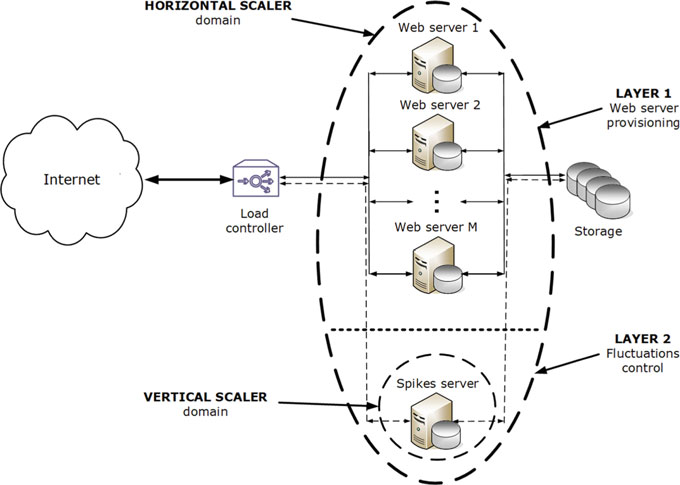
\includegraphics[width=\linewidth,height=.70\textheight,keepaspectratio]{../report/system.jpg}
    \source{Architettura adattata dal caso di studio in Serazzi, cap. 6.}
    \column{.41\textwidth}
    \tagbox{teal}{LAYER 1}\quad\textbf{Web Server pool}
    \begin{itemize}
      \item traffico ordinario;
      \item disciplina Processor Sharing;
      \item scaling orizzontale lento.
    \end{itemize}
    \vspace{0.25cm}
    \tagbox{coral}{LAYER 2}\quad\textbf{Spike Server}
    \begin{itemize}
      \item percorso ausiliario sempre disponibile;
      \item assorbe la congestione temporanea;
      \item scaling verticale immediato.
    \end{itemize}
    \vspace{0.25cm}
    {\small Il Load Controller sceglie il nodo e decide
      \textbf{evento per evento} se assegnarli
      il job o deviarlo.}
  \end{columns}
\end{frame}

% 4 ------------------------------------------------------------------------
\begin{frame}{Obiettivi e percorso sperimentale}
  \begin{columns}[T,onlytextwidth]
    \column{.31\textwidth}
    \begin{block}{1. Dimensionare}
      Routing, soglia di deviazione, incremento verticale e soglie
      dello scaling orizzontale.
    \end{block}
    \column{.31\textwidth}
    \begin{block}{2. Valutare}
      Trade-off costo--latenza, transitorio e robustezza alla burstiness.
    \end{block}
    \column{.31\textwidth}
    \begin{block}{3. Migliorare}
      Ridurre il chattering del router con un controllo a bande.
    \end{block}
  \end{columns}
  \vspace{0.55cm}
  \begin{tikzpicture}[node distance=.83cm, every node/.style={font=\scriptsize}]
    \node[rounded corners,fill=ink,text=white,minimum width=2.15cm,minimum height=.75cm] (m) {Modello};
    \node[rounded corners,fill=teal,text=white,minimum width=2.15cm,minimum height=.75cm,right=of m] (ve) {Verifica};
    \node[rounded corners,fill=green,text=white,minimum width=2.15cm,minimum height=.75cm,right=of ve] (va) {Validazione};
    \node[rounded corners,fill=gold,text=ink,minimum width=2.15cm,minimum height=.75cm,right=of va] (e) {Esperimenti};
    \node[rounded corners,fill=coral,text=white,minimum width=2.15cm,minimum height=.75cm,right=of e] (i) {Miglioramento};
    \draw[-{Latex},thick,muted] (m)--(ve);
    \draw[-{Latex},thick,muted] (ve)--(va);
    \draw[-{Latex},thick,muted] (va)--(e);
    \draw[-{Latex},thick,muted] (e)--(i);
  \end{tikzpicture}
\end{frame}

% --------------------------------------------------------------------------
\begin{frame}{Concettuale I: una rete di code gerarchica}
  \centering
  \resizebox{!}{.56\textheight}{%
    \begin{tikzpicture}[>=Stealth,line width=.8pt]
      \tikzset{
        lb/.style={circle,draw=teal,fill=teal!10,minimum size=1.45cm,
            font=\small\bfseries,align=center},
        srv/.style={circle,draw=cyan,fill=cyan!10,minimum size=.85cm,font=\small},
        spike/.style={circle,draw=coral,fill=coral!10,minimum size=.85cm,font=\small},
        flow/.style={-{Latex},draw=muted,thick},
        pipe/.style={draw=muted,thick}
      }
      \node[lb] (lb) at (0,0) {Load\\Controller};
      \coordinate (bus) at (2.0,0);
      \node[srv] (s1) at (5.5,2.6) {\(\mu_{web}\)};
      \node[srv] (s2) at (5.5,1.35) {\(\mu_{web}\)};
      \node at (4.65,.25) [text=muted,font=\Large\bfseries] {\(\vdots\)};
      \node[srv] (sn) at (5.5,-.75) {\(\mu_{web}\)};
      \node[spike] (ss) at (5.5,-2.65) {\(\mu_{spike}\)};

      \foreach \s in {s1,s2,sn}{
          \coordinate (q\s) at ([xshift=-1.1cm]\s.west);
          \draw[thick,color=cyan] (q\s) ++(0,.28)--++(1.1,0)--++(0,-.56)--++(-1.1,0);
          \draw[muted!70] (q\s) ++(0,.14)--++(1.1,0);
          \draw[muted!70] (q\s)--++(1.1,0);
          \draw[muted!70] (q\s) ++(0,-.14)--++(1.1,0);
        }

      \coordinate (qss) at ([xshift=-1.1cm]ss.west); 
      \draw[thick, color=coral] (qss) ++(0,.28)--++(1.1,0)--++(0,-.56)--++(-1.1,0);
      \draw[muted!70] (qss) ++(0,.14)--++(1.1,0);
      \draw[muted!70] (qss)--++(1.1,0);
      \draw[muted!70] (qss) ++(0,-.14)--++(1.1,0);

      \draw[flow] (-2,0)--node[above]{\(\lambda\)}(lb.west);
      \draw[pipe] (lb.east)--(bus);
      \draw[pipe] (2,2.6)--(2,-2.65);
      \draw[flow] (2,2.6)--(qs1);
      \draw[flow] (2,1.35)--(qs2);
      \draw[flow] (2,-.75)--(qsn);
      \draw[flow] (2,-2.65)--(qss);
      \draw[flow] (s1.east)--++(1.25,0);
      \draw[flow] (s2.east)--++(1.25,0);
      \draw[flow] (sn.east)--++(1.25,0);
      \draw[flow] (ss.east)--++(1.25,0);

      \begin{scope}[on background layer]
        \draw[cyan,dashed,fill=cyan!3,rounded corners=7pt,thick]
        (3.55,-1.35) rectangle (6.25,3.2);
        \draw[coral,dashed,fill=coral!3,rounded corners=7pt,thick]
        (3.55,-3.25) rectangle (6.25,-2.05);
      \end{scope}
      \node[cyan!70!ink,font=\small\bfseries] at (4.9,3.48) {Web Servers Pool};
      \node[coral!80!ink,font=\small\bfseries] at (4.9,-1.78) {Spike Server};
    \end{tikzpicture}}
  \vspace{0.12cm}
  \begin{center}
    \tagbox{teal}{N(t) STAZIONI PARALLELE}\qquad
    \tagbox{coral}{1 STAZIONE AUSILIARIA}\qquad
    \tagbox{ink}{PROCESSOR SHARING}
  \end{center}
\end{frame}

% --------------------------------------------------------------------------
\begin{frame}{Concettuale II: lo stato del sistema}
  \[
    \boxed{
      S(t)=\left\{
      N(t),\ \mathbf{n}(t),\ n_s(t),\ v_s(t),\
      \widehat{W}_{mw}(t),\ \tau_h(t),\ \tau_v(t)
      \right\}}
  \]
  \vspace{0.35cm}
  \begin{columns}[T,onlytextwidth]
    \column{.47\textwidth}
    \tagbox{teal}{STATO FISICO}
    \vspace{0.18cm}
    \begin{itemize}
      \item \(N(t)\): Web Server attivi;
      \item \(\mathbf n(t)=(n_1,\ldots,n_{N(t)})\): carico del pool;
      \item \(n_s(t)\): job sullo Spike Server;
      \item \(v_s(t)\): capacità istantanea dello Spike.
    \end{itemize}
    \column{.47\textwidth}
    \tagbox{coral}{MEMORIA DEL CONTROLLO}
    \vspace{0.18cm}
    \begin{itemize}
      \item \(\widehat W_{mw}(t)\): risposta media nella moving window;
      \item \(\tau_h(t)\): cooldown orizzontale residuo;
      \item \(\tau_v(t)\): cooldown verticale residuo.
    \end{itemize}
  \end{columns}
  \begin{block}{Transizioni}
    Arrivo, completamento e monitoraggio periodico.
  \end{block}
\end{frame}

% --------------------------------------------------------------------------
\begin{frame}{Concettuale III: Tre decisioni, tre scale di reazione}
  \begin{columns}[T,onlytextwidth]
    \column{.305\textwidth}
    \begin{block}{Routing}
      \centering
      \(\text{job}\leftrightarrow n_i < SI_{\max}\)
      \vspace{0.15cm}

      \tagbox{teal}{OGNI ARRIVO}
    \end{block}
    \begin{itemize}
      \item seleziona il nodo;
      \item devia oltre \(SI_{\max}\).
    \end{itemize}
    \column{.305\textwidth}
    \begin{block}{Scaling verticale}
      \centering
      \(v_s\leftrightarrow v_s+\Delta v_s\)
      \vspace{0.15cm}

      \tagbox{coral}{BREVE PERIODO}
    \end{block}
    \begin{itemize}
      \item osserva lo Spike Server;
      \item capacità immediata.
    \end{itemize}
    \column{.305\textwidth}
    \begin{block}{Scaling orizzontale}
      \centering
      \(N\leftrightarrow N\pm1\)
      \vspace{0.15cm}

      \tagbox{gold}{LUNGO PERIODO}
    \end{block}
    \begin{itemize}
      \item moving window di \(R_0\);
      \item scale out / scale in;
      \item cooldown.
    \end{itemize}
  \end{columns}
\end{frame}

% --------------------------------------------------------------------------
\begin{frame}{Specifiche I: workload e disciplina di servizio}
  \small
  \begin{columns}[T,onlytextwidth]
    \column{.48\textwidth}
    \tagbox{teal}{PROCESSO DI ARRIVO}
    \[
      T_j=A_j-A_{j-1},
      \qquad E[T]=\frac{1}{\lambda}
    \]
    \[
      T\sim
      \begin{cases}
        \mathrm{Exp}(m_1) & \text{con probabilità }p   \\
        \mathrm{Exp}(m_2) & \text{con probabilità }1-p
      \end{cases}
    \]
    \begin{itemize}
      \setlength{\itemsep}{1pt}
      \item \(H_2\) per rappresentare \(C_V^A>1\);
      \item \(\lambda\in[2,14]\) job/s;
      \item burstiness: \(C_V^A\in\{1,4,8,12\}\).
    \end{itemize}
    \column{.48\textwidth}
    \tagbox{coral}{PROCESSO DI SERVIZIO}
    \[
      S_j\sim H_2 =
      \begin{cases}
        \mathrm{Exp}(\nu_1) & \text{con probabilità }q\\
        \mathrm{Exp}(\nu_2) & \text{con probabilità }1-q
      \end{cases}
    \]
    \begin{itemize}
      \setlength{\itemsep}{1pt}
      \item \(S_j\) è la domanda di servizio del job \(j\);
      \item anche il servizio è iperesponenziale: \(C_V^S>1\).
    \end{itemize}
    \vspace{0.04cm}

    \tagbox{teal}{DISCIPLINA PROCESSOR SHARING}
    \[
      \mu_i^{job}(t)=\frac{\mu_i(t)}{n_i(t)},
      \qquad
      \mu_i(t)=\mu_{web}
    \]
    \[
      \mu_s^{job}(t)
      =\frac{v_s(t)\mu_{base}}{n_s(t)}
    \]
    {\footnotesize Servizio immediato e capacità equamente ripartita.}
  \end{columns}
\end{frame}

% --------------------------------------------------------------------------
\begin{frame}{Specifiche II: probabilità di routing}
  \small
  \begin{columns}[T,onlytextwidth]
    \column{.48\textwidth}
    \tagbox{teal}{WEB SERVER CANDIDATO}
    \par\vspace{0.06cm}
    La politica \(\pi_R\) sceglie un nodo ordinario \(i\).
    \[
      \lambda_i^{cand}=p_i\lambda,
      \qquad
      \sum_{i=1}^{N(t)}p_i=1
    \]
    \vspace{-0.08cm}
    \begin{itemize}
      \setlength{\itemsep}{0pt}
      \item RR / Random: \(p_i\) uniforme o uniforme in media;
      \item Least Loaded / Po2C: \(p_i\) dipende dallo stato.
    \end{itemize}
    \vspace{0.10cm}
    \tagbox{coral}{DEVIAZIONE EVENTUALE}
    \[
      d_i(t)=
      \begin{cases}
        1 & SI_i(t)\ge SI_{\max}\\
        0 & SI_i(t)<SI_{\max}
      \end{cases}
    \]
    \vspace{-0.06cm}
    {\footnotesize \(d_i(t)=1\): il job candidato per \(i\) va allo Spike Server.}

    \column{.48\textwidth}
    \tagbox{violet}{FLUSSI EFFETTIVI}
    \par\vspace{0.06cm}
    \(q_i\): probabilità osservata di dirottamento per il candidato \(i\).
    \[
      \lambda_i=(1-q_i)p_i\lambda,
      \qquad
      \lambda_s=\sum_{i=1}^{N(t)}q_i p_i\lambda
    \]
    \vspace{-0.05cm}
    \begin{center}
    \begin{tikzpicture}[scale=.86, transform shape,
      node distance=0.58cm,
      flow/.style={draw=black!12, rounded corners=5pt, fill=black!3,
        minimum width=2.65cm, minimum height=.56cm, align=center,
        font=\scriptsize},
      arrow/.style={-{Latex[length=2mm]}, thick, draw=black!45}
    ]
      \node[flow, fill=teal!12] (arr) {arrivi\\\(\lambda\)};
      \node[flow, fill=teal!8, below=of arr] (cand) {candidato\\\(p_i\lambda\)};
      \node[flow, fill=coral!12, below left=.55cm and -.2cm of cand] (web) {Web \(i\)\\\((1-q_i)p_i\lambda\)};
      \node[flow, fill=violet!13, below right=.55cm and -.2cm of cand] (spike) {Spike\\\(q_i p_i\lambda\)};
      \draw[arrow] (arr) -- (cand);
      \draw[arrow] (cand) -- (web);
      \draw[arrow] (cand) -- (spike);
    \end{tikzpicture}
    \end{center}
    \vspace{-0.18cm}
    \[
      D_{spike}=\frac{X_{spike}}{X_0}
      \simeq \frac{\lambda_s}{\lambda}
    \]
    \vspace{-0.08cm}
    {\footnotesize Il routing non cambia \(\lambda\): redistribuisce solo il carico.}
  \end{columns}
\end{frame}

% --------------------------------------------------------------------------
\begin{frame}{Specifiche III: parametri fissati del controllo}
  \begin{columns}[T,onlytextwidth]
    \column{.54\textwidth}
      \tagbox{teal}{LEGAMI CON \(SI_{\max}\)}
      \vspace{0.25cm}
      \[
        W=2.5\,SI_{\max}
      \]
      \[
        L_{sv}^{\max}=\frac{SI_{\max}}{2.5},
        \qquad
        L_{sv}^{\min}=0.7\,L_{sv}^{\max}
      \]
      \vspace{0.2cm}
      {\small La finestra orizzontale e le soglie dello scaler verticale
      restano proporzionate alla congestione ammessa sul Web Server.}
    \column{.42\textwidth}
      \begin{block}{Con \(SI_{\max}=40\)}
        \centering
        \vspace{0.12cm}
        {\Large\bfseries \(W=100\)}\par
        {\scriptsize completamenti nella moving window}
        \vspace{0.35cm}

        {\Large\bfseries \(L_{sv}^{\max}=16\)}\par
        {\scriptsize soglia di Speed Up}
        \vspace{0.35cm}

        {\Large\bfseries \(L_{sv}^{\min}=11.2\)}\par
        {\scriptsize soglia di Speed Down}
        \vspace{0.1cm}
      \end{block}
  \end{columns}
  \vspace{0.35cm}
  \begin{center}
    \tagbox{coral}{VALORI FISSATI A PRIORI}\qquad
    {\small non appartengono alla successiva campagna di tuning}
  \end{center}
\end{frame}

% --------------------------------------------------------------------------
\begin{frame}[fragile=singleslide]{Computazionale I: oggetti di dominio e Processor Sharing}
  \begin{columns}[T,onlytextwidth]
    \column{.54\textwidth}
    \resizebox{.90\linewidth}{!}{%
      \begin{tikzpicture}[
          every node/.style={font=\scriptsize},
          uml/.style={rectangle,draw=teal,fill=teal!5,
              minimum width=3.25cm,minimum height=.92cm,align=center}]
        \node[uml,draw=ink,fill=ink!5] (server) at (3.2,2.0)
          {\textbf{\texttt{Server}}\\\rule{2.8cm}{.25pt}\\activeJobs, speedMultiplier};
        \node[uml] (web) at (1.5,.15)
          {\textbf{\texttt{WebServer}}\\\rule{2.8cm}{.25pt}\\getSpikeIndicator()};
        \node[uml,draw=coral,fill=coral!5] (spike) at (4.9,.15)
          {\textbf{\texttt{SpikeServer}}\\\rule{2.8cm}{.25pt}\\};
        \node[uml,draw=cyan,fill=cyan!5] (cluster) at (1.5,-1.55)
          {\textbf{\texttt{WebServerCluster}}\\\rule{2.8cm}{.25pt}\\active, draining, all};

        \draw[-{Triangle[open]},thick,muted] (web.north)--(server.south west);
        \draw[-{Triangle[open]},thick,muted] (spike.north)--(server.south east);
        \draw[thick,muted] (cluster.north)--node[right,font=\tiny]{\(1..*\)}(web.south);
        \node[diamond,draw=muted,fill=white,minimum size=7pt,inner sep=0pt]
          at (cluster.north) {};
      \end{tikzpicture}
    }
    \vspace{0.22cm}
    \begin{lstlisting}[style=slidecode]
double work = elapsed * speedMultiplier / activeJobs.size();
for (Job job : activeJobs) {
    job.decreaseRemainingDemand(work);
}
      \end{lstlisting}
    \column{.42\textwidth}
    \tagbox{teal}{NUCLEO PS}
    \[
      \Delta w_j=\frac{s\,\Delta t}{|\text{activeJobs}|}
    \]
    \begin{itemize}
      \setlength{\itemsep}{2pt}
      \item ogni job entra subito in servizio;
      \item la domanda residua viene aggiornata a ogni evento;
      \item lo scale-in sposta il server in \emph{draining};
      \item i job già assegnati terminano senza perdite.
    \end{itemize}
    \vspace{-0.13cm}
    \begin{block}{Draining Server}
      Un server rimosso non riceve nuovi job, ma resta operativo finché
      non si svuota.
    \end{block}
  \end{columns}
\end{frame}

% --------------------------------------------------------------------------
\begin{frame}[fragile=singleslide]{Computazionale II: motore next-event}
  \begin{columns}[T,onlytextwidth]
    \column{.58\textwidth}
    \resizebox{.82\linewidth}{!}{%
      \begin{tikzpicture}[
          node distance=.22cm,
          every node/.style={font=\scriptsize},
          flowstep/.style={rounded corners,fill=paper,draw=teal,
              minimum width=5.9cm,minimum height=.58cm,align=center}]
        \node[flowstep] (a) {1. Estrai il primo evento dalla \texttt{PriorityQueue}};
        \node[flowstep,below=of a] (b) {2. Avanza il lavoro di tutti i job fino a \(t_{next}\)};
        \node[flowstep,below=of b] (c) {3. Aggiorna clock e stato};
        \node[flowstep,below=of c] (d) {4. Gestisci arrivo, completamento o monitoraggio};
        \node[flowstep,below=of d] (e) {5. Rischedula i completamenti interessati};
        \foreach \x/\y in {a/b,b/c,c/d,d/e}
        \draw[-{Latex},thick,muted] (\x)--(\y);
      \end{tikzpicture}
    }
    \vspace{0.18cm}
    \begin{lstlisting}[style=slidecode]
if (eventQueue.isEmpty()) return false;

Event event = eventQueue.poll();
double nextTime = event.getTime();

processActiveJobs(nextTime - clock, nextTime);
clock = nextTime;
processEvent(event);
return true;
      \end{lstlisting}
    \column{.38\textwidth}
    \tagbox{coral}{FUTURE EVENT LIST}
    \vspace{0.25cm}
    \[
      t_j^{comp}
      =t+\frac{d_j\,n(t)}{s}
    \]
    \begin{itemize}
      \item arrivo: cambia \(n(t)\);
      \item completamento: cambia \(n(t)\);
      \item speed up/down: cambia \(s\);
      \item ogni variazione modifica le date future.
    \end{itemize}
    \vspace{0.2cm}
    {\small Il clock salta direttamente al prossimo evento: nessun passo
      temporale artificiale.}
  \end{columns}
\end{frame}

% --------------------------------------------------------------------------
\begin{frame}[fragile=singleslide]{Computazionale III: routing e autoscaler componibili}
  \begin{columns}[T,onlytextwidth]
    \column{.58\textwidth}
    \resizebox{\linewidth}{!}{%
      \begin{tikzpicture}[
          every node/.style={font=\scriptsize},
          uml/.style={rectangle,draw=teal,fill=teal!5,
              minimum width=2.75cm,minimum height=.86cm,align=center}]
        \node[uml,draw=ink,fill=ink!5] (lm) at (4.3,2.2)
          {\textbf{\texttt{LoadManager}}\\\rule{2.3cm}{.25pt}\\router, hScaler, vScaler};
        \node[uml] (router) at (1.3,.45)
          {\textbf{\texttt{Router}}\\\rule{2.3cm}{.25pt}\\route(job, cluster)};
        \node[uml,draw=cyan,fill=cyan!5] (hs) at (4.3,.45)
          {\textbf{\texttt{HorizontalScaler}}\\\rule{2.3cm}{.25pt}\\evaluateScaling()};
        \node[uml,draw=coral,fill=coral!5] (vs) at (7.3,.45)
          {\textbf{\texttt{VerticalScaler}}\\\rule{2.3cm}{.25pt}\\evaluateScaling()};

        \node[uml,minimum width=2.75cm] (strategy) at (1.3,-1.35)
          {\(\langle\!\langle\)strategy\(\rangle\!\rangle\)\\WS + Spike routing};
        \node[uml,draw=cyan,fill=cyan!5,minimum width=2.75cm] (mh) at (4.3,-1.35)
          {\texttt{MovingWindow}\\HorizontalScaler};
        \node[uml,draw=coral,fill=coral!5,minimum width=2.75cm] (lv) at (7.3,-1.35)
          {\texttt{LoadThreshold}\\VerticalScaler};

        \foreach \n in {router,hs,vs}{
          \draw[thick,muted] (lm.south)--(\n.north);
          \node[diamond,draw=muted,fill=white,minimum size=5pt,inner sep=0pt]
            at (lm.south) {};
        }
        \draw[thick,muted] (router)--(strategy);
        \node[diamond,draw=muted,fill=white,minimum size=5pt,inner sep=0pt]
          at (router.south) {};
        \draw[-{Triangle[open]},thick,muted] (mh)--(hs);
        \draw[-{Triangle[open]},thick,muted] (lv)--(vs);
      \end{tikzpicture}
    }
    \vspace{0.18cm}
    \begin{lstlisting}[style=slidecode]
WebServer target = wsStrategy.selectWebServer(job, cluster);
if (spikeStrategy.shouldRouteToSpike(target, siMax)) {
    return spikeServer;
}

return target;
      \end{lstlisting}
    \column{.38\textwidth}
    \textbf{Separazione delle responsabilità}
    \begin{itemize}
      \item il motore non conosce la politica concreta;
      \item strategie sostituibili a configurazione invariata;
      \item scaler disattivabili con implementazioni \texttt{NoOp};
      \item controllo invocato dopo gli eventi e periodicamente.
    \end{itemize}
    \vspace{0.25cm}
    \begin{block}{Modularità}
      Routing e scaler possono essere isolati, confrontati e verificati
      senza modificare il controller.
    \end{block}
  \end{columns}
\end{frame}

% --------------------------------------------------------------------------
\begin{frame}[fragile=singleslide]{Computazionale IV: Batch Means e repliche indipendenti}
  \begin{columns}[T,onlytextwidth]
    \column{.31\textwidth}
    \begin{block}{Builder}
      \texttt{SimulationBuilder}

      Componenti dalla configurazione.
    \end{block}
    \column{.31\textwidth}
    \begin{block}{Facade}
      \texttt{SimulationFacade}

      Batch Means e repliche indipendenti.
    \end{block}
    \column{.31\textwidth}
    \begin{block}{Collector}
      Decorator

      Serie, checkpoint, CSV e JSON.
    \end{block}
  \end{columns}
  \vspace{0.34cm}
  \begin{columns}[T,onlytextwidth]
    \column{.49\textwidth}
    \tagbox{teal}{BATCH MEANS}
    \begin{lstlisting}[style=slidecode]
Simulator controller = builder.build();

if (warmUpJobs > 0) {
    controller.run(untilJobsCompleted(warmUpJobs));
}

controller.resetStatistics();

for (int i = 0; i < numBatches; i++) {
    controller.run(untilJobsCompleted(batchSize));
    updateAggregators(controller);
    controller.resetStatistics();
}
      \end{lstlisting}
      {\scriptsize Un solo sistema evolve nel tempo; ogni batch produce
        un'osservazione dopo il warm-up.}
    \column{.49\textwidth}
    \tagbox{coral}{REPLICHE INDIPENDENTI}
    \begin{lstlisting}[style=slidecode]
long currentSeed = config.execution().seed();

for (int i = 0; i < numReplications; i++) {
    Simulator controller = new SimulationBuilder()
        .config(config.withSeed(currentSeed))
        .build();

    controller.run(untilTimeElapsed(maxTime));
    updateAggregators(controller);

    // Stream successivo, non riuso lo stesso seed
    currentSeed = controller.getSeed();
}
      \end{lstlisting}
      {\scriptsize Ogni replica ricostruisce il sistema; il seed finale
        della run diventa il seed iniziale della successiva.}
  \end{columns}
\end{frame}

% 6 ------------------------------------------------------------------------
% \begin{frame}{Orizzonte di studio: finito e stazionario}
%   \begin{columns}[T,onlytextwidth]
%     \column{.47\textwidth}
%     \tagbox{coral}{ORIZZONTE FINITO}
%     \vspace{0.15cm}
%     \begin{itemize}
%       \item sistema inizialmente vuoto;
%       \item repliche indipendenti;
%       \item medie cumulative nel tempo;
%       \item misura dell'assestamento iniziale.
%     \end{itemize}
%     \vspace{0.3cm}
%     \textbf{Perché?} È il comportamento percepito durante l'avvio e
%     dimostra se il sistema converge.
%     \column{.47\textwidth}
%     \tagbox{teal}{STATO STAZIONARIO}
%     \vspace{0.15cm}
%     \begin{itemize}
%       \item warm-up derivato dalla convergenza;
%       \item Batch Means;
%       \item batch dimensionati tramite ACF;
%       \item intervalli di confidenza al 95\%.
%     \end{itemize}
%     \vspace{0.3cm}
%     \textbf{Perché?} Serve a confrontare configurazioni di lungo periodo
%     rimuovendo il bias iniziale.
%   \end{columns}
%   \vspace{0.45cm}
%   \begin{center}
%     \metric{\(5\times\)}{fattore prudenziale sul warm-up}{coral}
%     \hfill
%     \metric{\(|\rho_1|<0.1\)}{target di autocorrelazione lag-1}{teal}
%     \hfill
%     \metric{95\%}{livello di confidenza}{cyan}
%   \end{center}
% \end{frame}

% 7 ------------------------------------------------------------------------
% \begin{frame}{Credibilità del simulatore: verifica e validazione}
%   \begin{columns}[T,onlytextwidth]
%     \column{.48\textwidth}
%     \textbf{Verifica interna}
%     \begin{itemize}
%       \item casi M/M/1 confrontati con risultati analitici;
%       \item Legge di Little e conservazione del flusso;
%       \item trace deterministiche per routing e scaler;
%       \item test con workload \(H_2/H_2/1\).
%     \end{itemize}
%     \column{.48\textwidth}
%     \textbf{Validazione esterna con JMT}
%     \vspace{0.2cm}
%     \renewcommand{\arraystretch}{1.25}
%     \begin{tabular}{@{}lrr@{}}
%       \toprule
%       \textbf{Metrica} & \textbf{Java} & \textbf{Scarto} \\
%       \midrule
%       Throughput       & --            & \(0.34\%\)      \\
%       Job medi         & --            & \(0.46\%\)      \\
%       \(R_0\)          & \(0.8998\,s\) & \(0.50\%\)      \\
%       \bottomrule
%     \end{tabular}
%     \vspace{0.35cm}
% 
%     {\small Gli intervalli di confidenza delle due implementazioni
%       indipendenti si sovrappongono.}
%   \end{columns}
%   \vspace{0.5cm}
%   \begin{block}{Esito}
%     Il motore riproduce correttamente sia i casi con soluzione nota sia
%     l'architettura Web Server--Spike Server.
%   \end{block}
% \end{frame}

% --------------------------------------------------------------------------
\begin{frame}{Verifica: il routing segue esattamente la soglia}
  \begin{columns}[T,onlytextwidth]
    \column{.67\textwidth}
    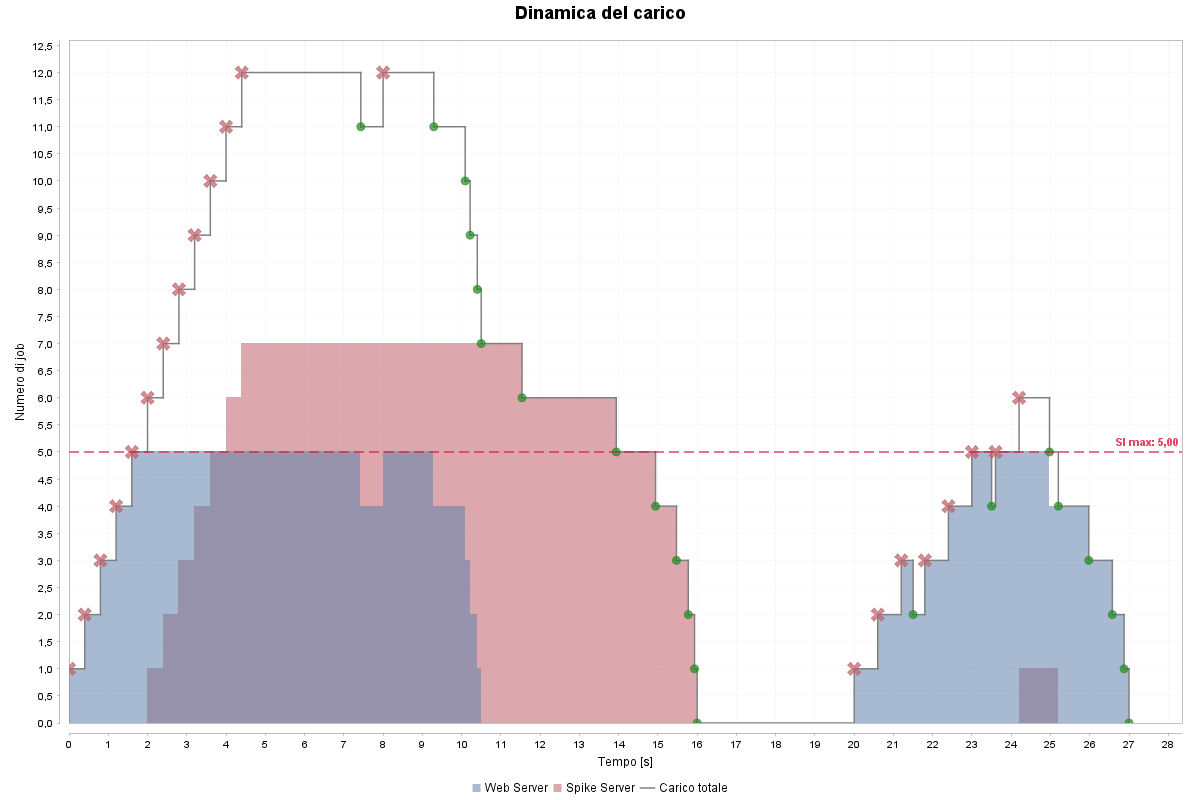
\includegraphics[width=\linewidth,height=.70\textheight,keepaspectratio]{../data/vv/chart/spike_diversion_chart.png}
    \source{Job sul Web Server e deviazioni verso lo Spike Server.}
    \column{.30\textwidth}
    \tagbox{teal}{TRACE-DRIVEN}
    \vspace{0.35cm}
    \begin{itemize}
      \item arrivi noti;
      \item servizi noti;
      \item soglia nota;
      \item destinazione attesa nota.
    \end{itemize}
    \vspace{0.35cm}
    \begin{center}
      \metric{\(21\)}{job totali}{teal}
      \metric{\(8\)}{job deviati}{coral}
    \end{center}
    \vspace{0.35cm}

    {\small Nessuna perdita e nessun job già assegnato viene interrotto.}
  \end{columns}
\end{frame}

% --------------------------------------------------------------------------
\begin{frame}[shrink=2]{Verifica: gli scaler rispettano soglie e cooldown}
  \begin{columns}[T,onlytextwidth]
    \column{.49\textwidth}
    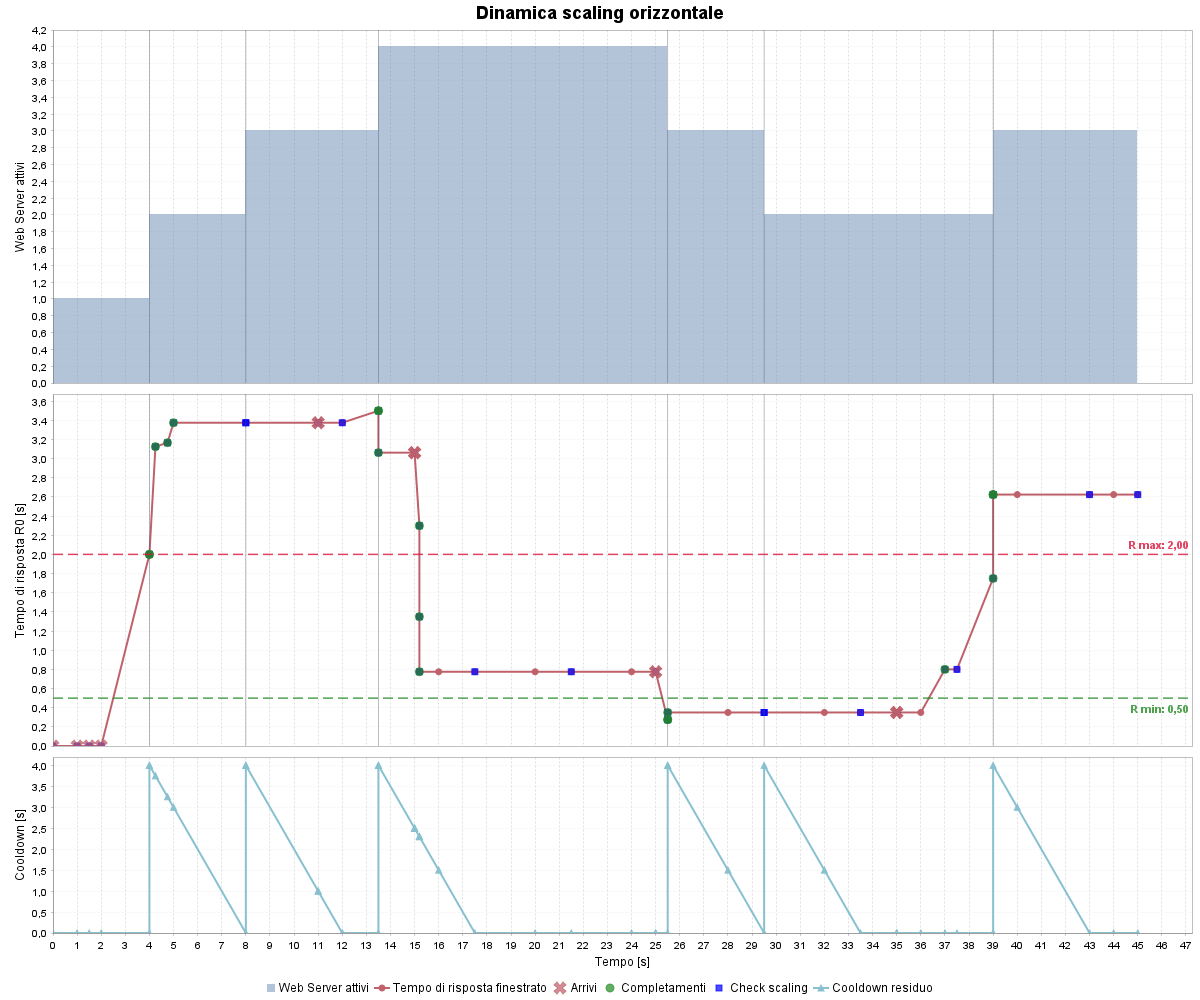
\includegraphics[width=\linewidth,height=.58\textheight,keepaspectratio]{../data/vv/chart/scaling/horizontal_scaling_chart.png}
    \begin{center}\tagbox{teal}{SCALING ORIZZONTALE}\end{center}
    {\scriptsize\centering Moving window, scale out/in e blocco nel cooldown.\par}
    \column{.49\textwidth}
    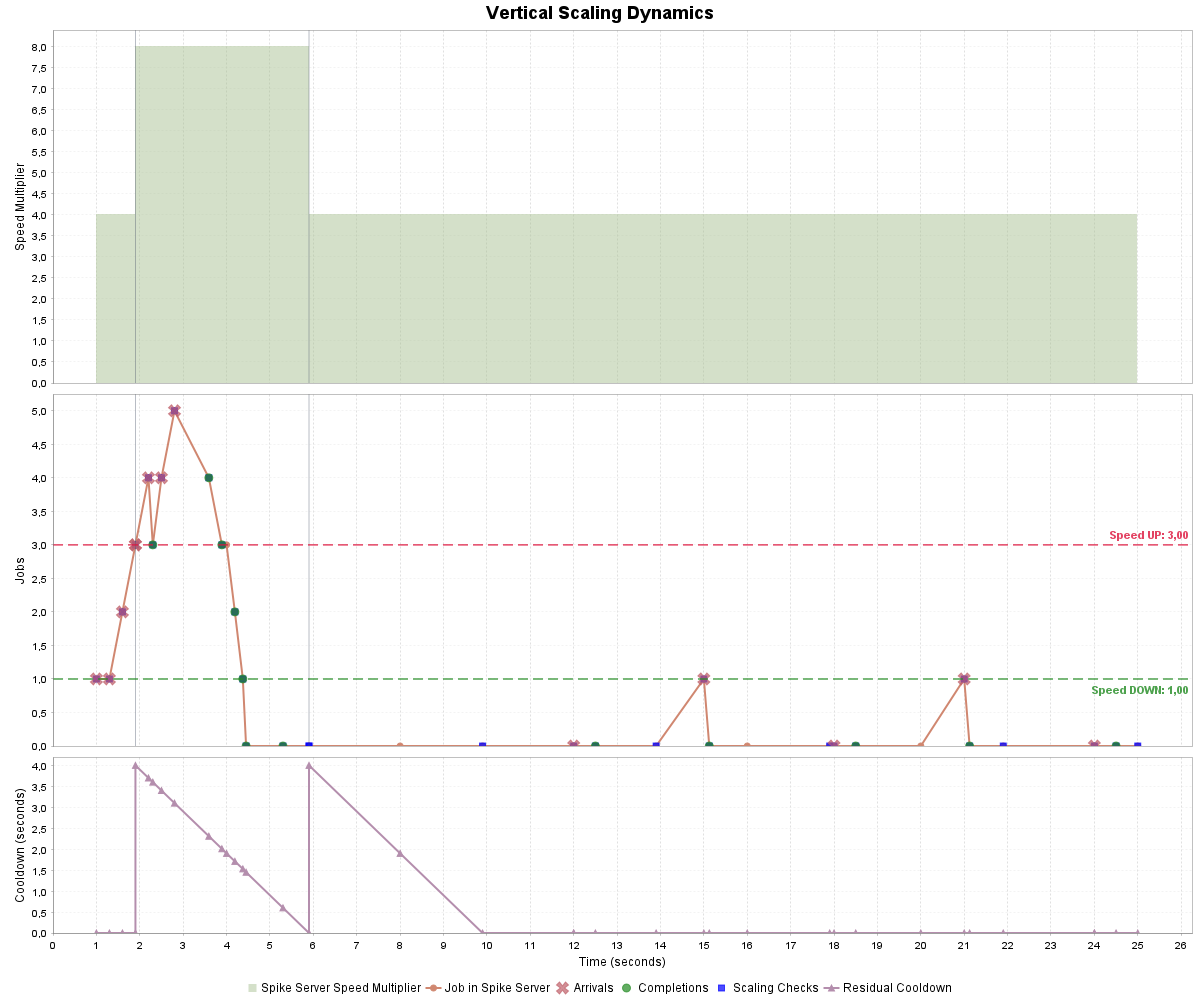
\includegraphics[width=\linewidth,height=.58\textheight,keepaspectratio]{../data/vv/chart/scaling/vertical_scaling_chart.png}
    \begin{center}\tagbox{coral}{SCALING VERTICALE}\end{center}
    {\scriptsize\centering Speed up a \(t=1.6\,s\), speed down a \(t=5.6\,s\).\par}
  \end{columns}
  \vspace{0.25cm}
  \begin{center}
    {\small Le transizioni osservate coincidono con gli istanti previsti
      dalle tracce deterministiche.}
  \end{center}
\end{frame}

% --------------------------------------------------------------------------
\begin{frame}{Validazione esterna: simulatore Java vs JMT}
  \vspace{-0.08cm}
  \begin{minipage}{\textwidth}
    \begin{minipage}[c]{.68\textwidth}
      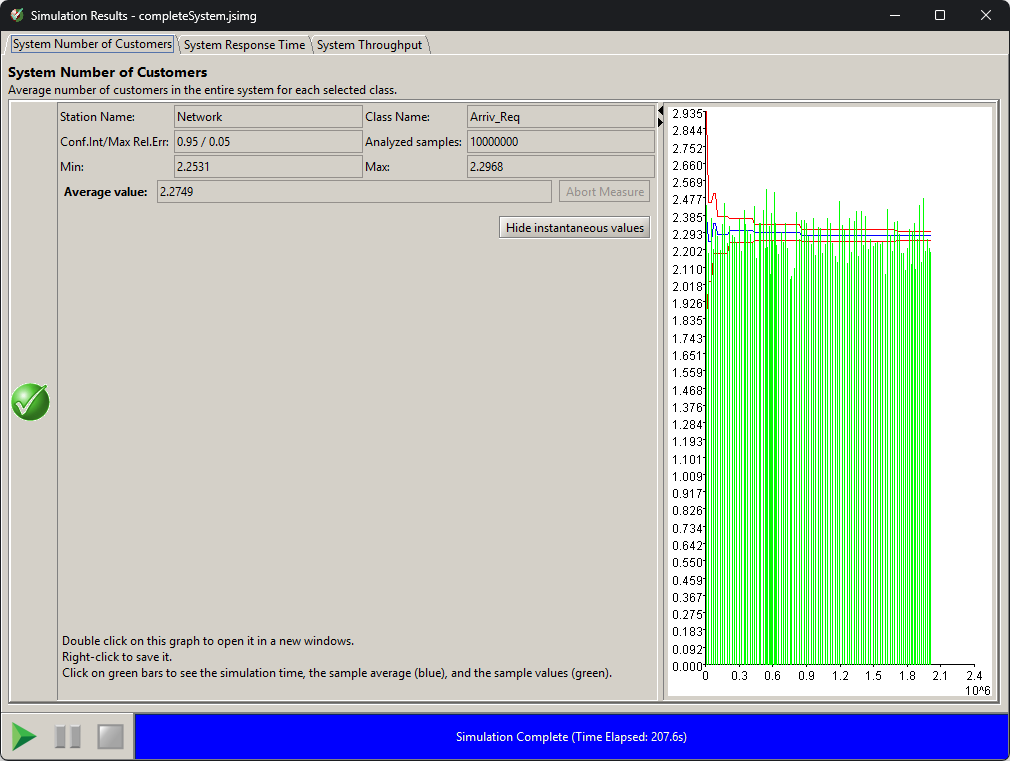
\includegraphics[
        width=\linewidth,
        trim=0 380 0 25,
        clip
      ]{../data/simulation/simple_system/job.png}
    \end{minipage}
    \hfill
    \begin{minipage}[c]{.28\textwidth}
      \tagbox{cyan}{JOB MEDI}\par
      \vspace{0.08cm}
      {\color{cyan}\LARGE \(0.46\%\)}\par
      {\footnotesize scarto sui job medi}
    \end{minipage}
    \vspace{0.03cm}

    \begin{minipage}[c]{.68\textwidth}
      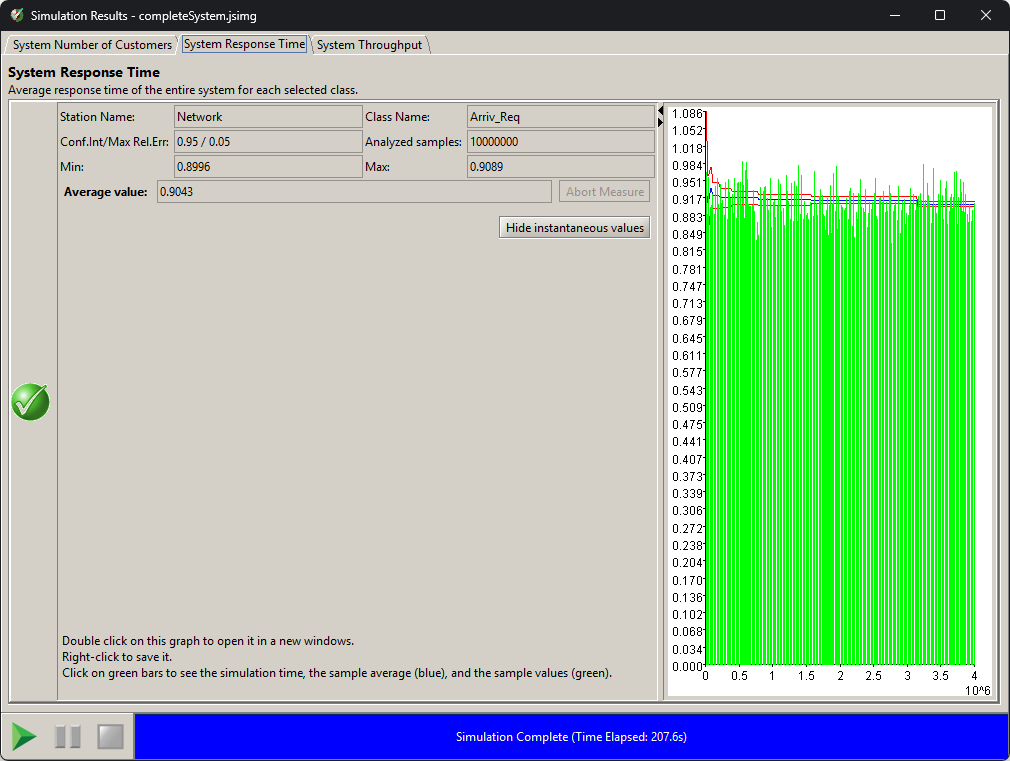
\includegraphics[
        width=\linewidth,
        trim=0 380 0 25,
        clip
      ]{../data/simulation/simple_system/response.png}
    \end{minipage}
    \hfill
    \begin{minipage}[c]{.28\textwidth}
      \tagbox{coral}{TEMPO DI RISPOSTA}\par
      \vspace{0.08cm}
      {\color{coral}\LARGE \(0.50\%\)}\par
      {\footnotesize scarto su \(R_0\)}
    \end{minipage}
    \vspace{0.03cm}

    \begin{minipage}[c]{.68\textwidth}
      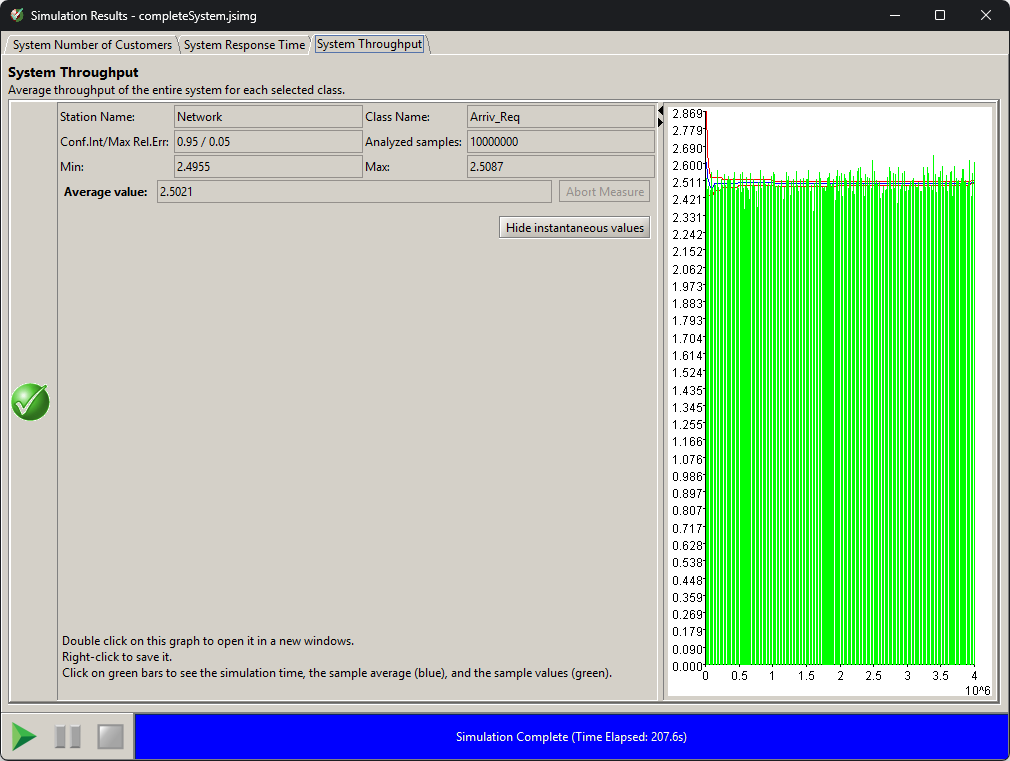
\includegraphics[
        width=\linewidth,
        trim=0 380 0 25,
        clip
      ]{../data/simulation/simple_system/throughput.png}
    \end{minipage}
    \hfill
    \begin{minipage}[c]{.28\textwidth}
      \tagbox{violet}{THROUGHPUT}\par
      \vspace{0.08cm}
      {\color{violet}\LARGE \(0.34\%\)}\par
      {\footnotesize scarto sul throughput}
    \end{minipage}
  \end{minipage}
  \source{Stesso workload e stessa disciplina; gli intervalli di confidenza si sovrappongono.}
\end{frame}

% 8 ------------------------------------------------------------------------
\begin{frame}{Obiettivo 1A: scegliere la politica di routing}
  \begin{columns}[T,onlytextwidth]
    \column{.64\textwidth}
    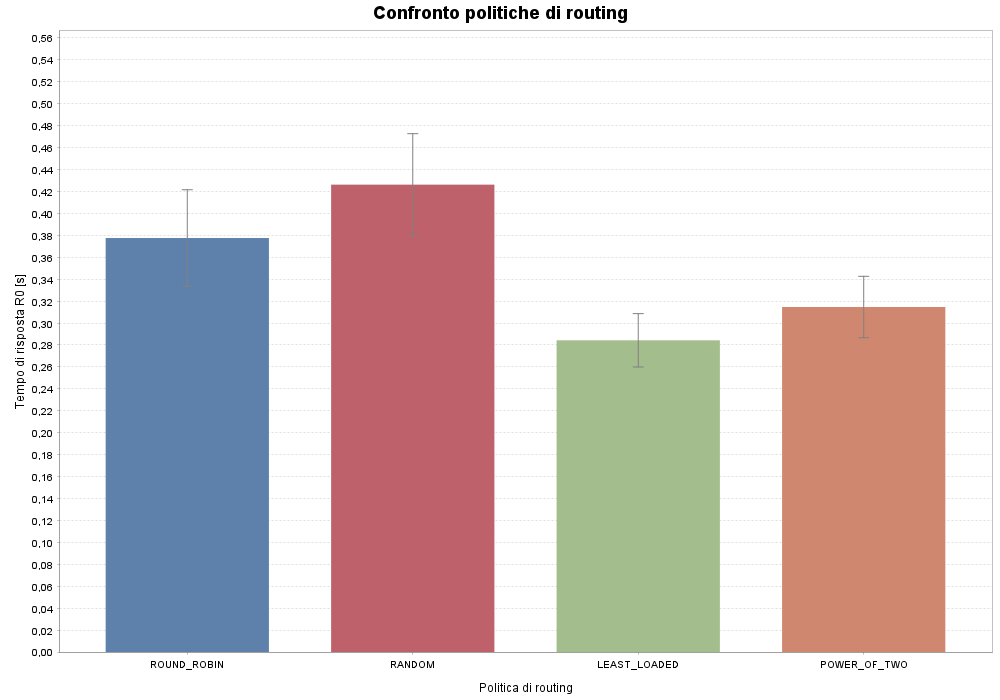
\includegraphics[width=\linewidth,height=.70\textheight,keepaspectratio]{../data/objective/routing_policy_comparison.png}
    \source{\(4\) Web Server, \(H_2/H_2\), \(\lambda=5\), \(C_V=4\).}
    \column{.33\textwidth}
    \tagbox{teal}{SCELTA}\par\vspace{0.12cm}
    {\Large\bfseries Least Loaded}
    \vspace{0.45cm}
    \begin{itemize}
      \item \(R_0=0.2843\,s\);
      \item \(-24.7\%\) vs Round Robin;
      \item \(-33.3\%\) vs Random;
      \item minima dispersione: \(\sigma=0.0243\,s\).
    \end{itemize}
    \vspace{0.35cm}
    {\small Osservare il carico istantaneo evita micro-congestioni che
      il Processor Sharing, da solo, non elimina.}
  \end{columns}
\end{frame}

% --------------------------------------------------------------------------
\begin{frame}{Obiettivo 1B: calibrare la soglia di deviazione}
  \begin{columns}[T,onlytextwidth]
    \column{.66\textwidth}
    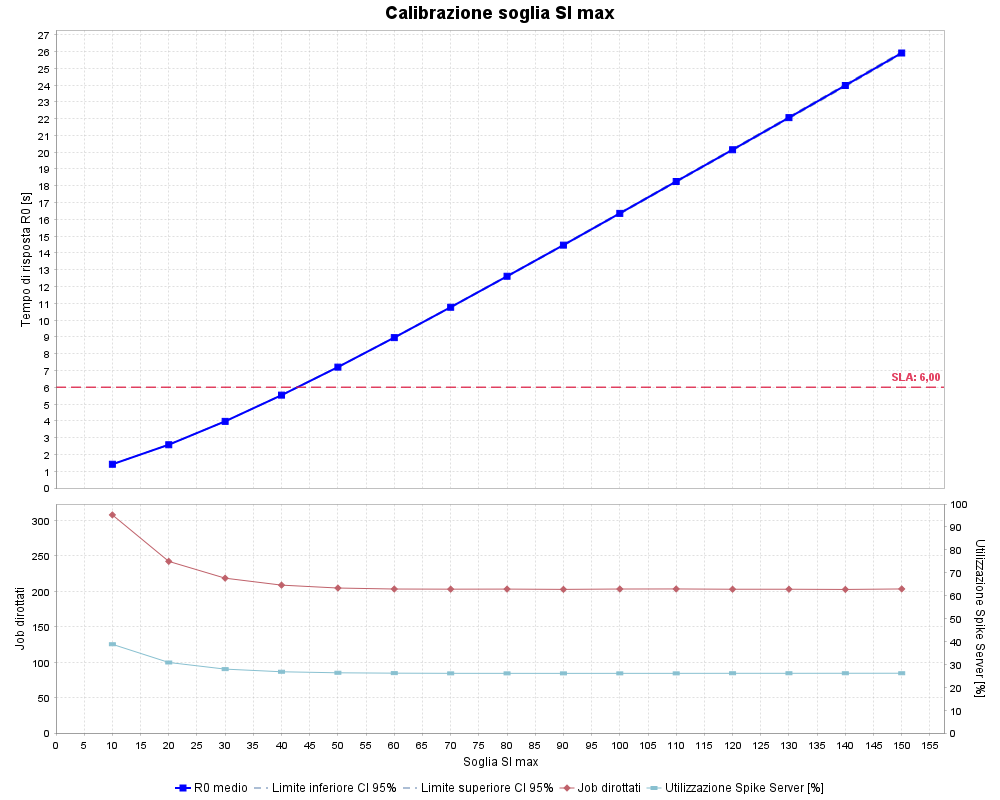
\includegraphics[width=\linewidth,height=.70\textheight,keepaspectratio]{../data/objective/simax_estimation.png}
    \source{Un Web Server, Spike Server attivo, \(H_2/H_2\), scaling disabilitato.}
    \column{.31\textwidth}
    \tagbox{teal}{SCELTA}\par\vspace{0.12cm}
    {\Large\bfseries \(SI_{\max}=40\)}
    \vspace{0.35cm}
    \begin{itemize}
      \item \(R_0=5.4209\,s\);
      \item CI \([5.3970,5.4448]\);
      \item job deviati: \(20.34\%\);
      \item utilizzo Spike: \(26.77\%\).
    \end{itemize}
    \vspace{0.25cm}
    \begin{block}{Il punto di rottura}
      A \(SI_{\max}=50\): \(R_0=7.0903\,s\). SLA violato.
    \end{block}
  \end{columns}
\end{frame}

% --------------------------------------------------------------------------
\begin{frame}{Obiettivo 1C: dimensionare lo scaling verticale}
  \begin{columns}[T,onlytextwidth]
    \column{.66\textwidth}
    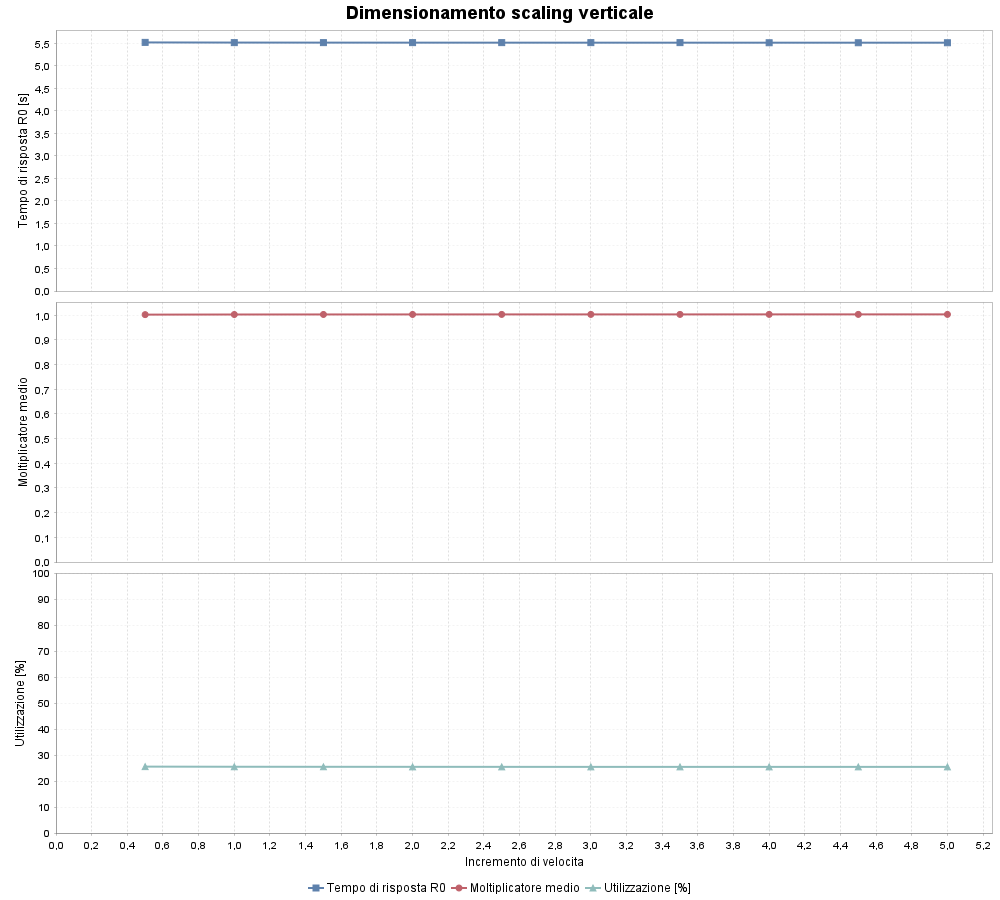
\includegraphics[width=\linewidth,height=.70\textheight,keepaspectratio]{../data/objective/vertical_step_sizing.png}
    \source{\(SI_{\max}=40\); incremento additivo di capacità variato da \(0.5\) a \(5.0\).}
    \column{.31\textwidth}
    \tagbox{teal}{SCELTA}\par\vspace{0.12cm}
    {\Large\bfseries \(\Delta v_s=1.0\)}
    \vspace{0.4cm}
    \begin{itemize}
      \item \(R_0\) resta tra \(5.4046\) e \(5.4109\,s\);
      \item tutti i CI al 95\% si sovrappongono;
      \item più capacità non produce un beneficio misurabile.
    \end{itemize}
    \vspace{0.3cm}
    {\small La capacità passa da \(1.0\) a \(2.0\): il raddoppio più
      sobrio, senza sovradimensionamento.}
  \end{columns}
\end{frame}

% 9 ------------------------------------------------------------------------
\begin{frame}{Obiettivo 1D: tracciare la frontiera orizzontale}
  \begin{columns}[T,onlytextwidth]
    \column{.67\textwidth}
    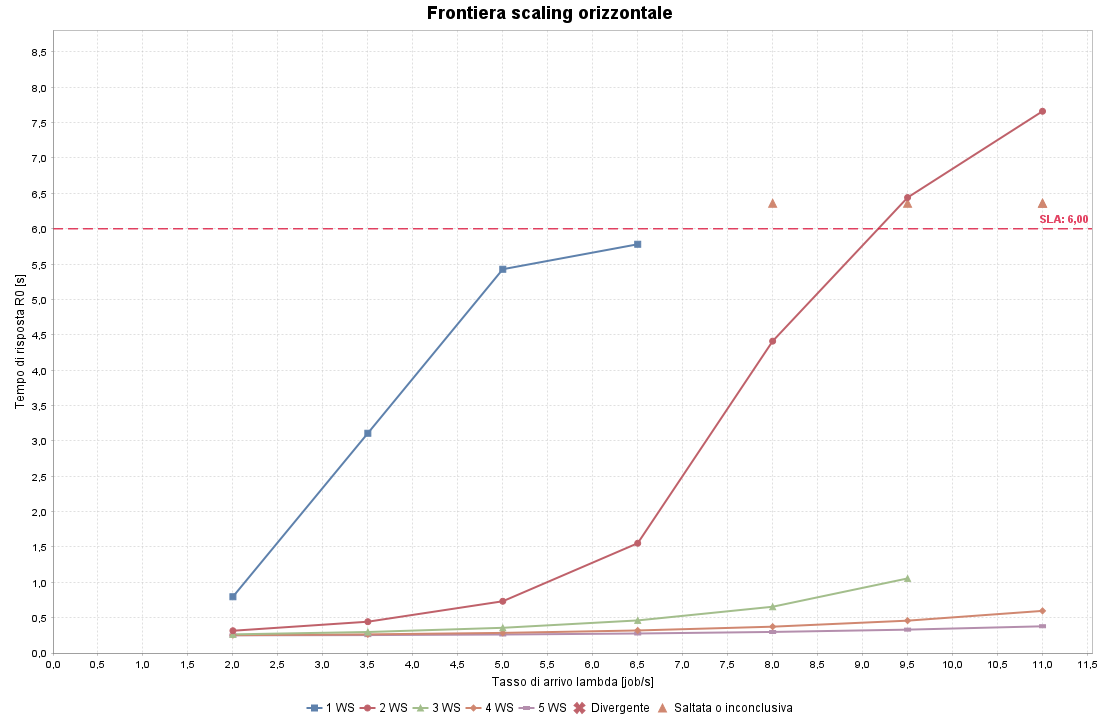
\includegraphics[width=\linewidth,height=.70\textheight,keepaspectratio]{../data/objective/horizontal_parameter_estimation.png}
    \source{Frontiera statica di capacità; SLA \(R_0\le6\,s\).}
    \column{.30\textwidth}
    \tagbox{teal}{SCELTA NOMINALE}\par\vspace{0.12cm}
    {\Large\bfseries \(R^{\min}=3.5\,s\)}
    \vspace{0.25cm}
    \begin{itemize}
      \item \(R^{\max}=6\,s\): coincide con lo SLA;
      \item a \(\lambda=5\), 1 WS: \(5.4271\,s\);
      \item a \(\lambda=11\), 3 WS: \(2.2695\,s\);
      \item a \(\lambda=11\), 2 WS: \(7.6609\,s\).
    \end{itemize}
    \vspace{0.2cm}
    {\small Per workload persistentemente aggressivi conviene
      \(R^{\min}\in[1.5,2.0]\,s\).}
  \end{columns}
\end{frame}

% --------------------------------------------------------------------------
\begin{frame}{Dimensionamento completato: la baseline}
  \begin{center}
    \begin{tikzpicture}[node distance=.22cm,every node/.style={font=\small}]
      \node[rounded corners,fill=ink,text=white,minimum width=3.0cm,
        minimum height=1.05cm,align=center] (r) {\textbf{Routing}\\Least Loaded};
      \node[rounded corners,fill=teal,text=white,minimum width=3.0cm,
        minimum height=1.05cm,align=center,right=of r] (s) {\textbf{Deviazione}\\\(SI_{\max}=40\)};
      \node[rounded corners,fill=cyan,text=white,minimum width=3.0cm,
        minimum height=1.05cm,align=center,right=of s] (v) {\textbf{Verticale}\\\(\Delta v_s=1.0\)};
      \node[rounded corners,fill=coral,text=white,minimum width=3.0cm,
        minimum height=1.05cm,align=center,right=of v] (h) {\textbf{Orizzontale}\\\(6.0/3.5\,s\)};
      \draw[-{Latex},thick,muted] (r)--(s);
      \draw[-{Latex},thick,muted] (s)--(v);
      \draw[-{Latex},thick,muted] (v)--(h);
    \end{tikzpicture}
  \end{center}
  \vspace{0.7cm}
  \begin{columns}[T,onlytextwidth]
    \column{.30\textwidth}
    \begin{block}{Osservazione}
      Finestra mobile: \(100\) completamenti.
    \end{block}
    \column{.30\textwidth}
    \begin{block}{Reazione}
      Cooldown iniziale: \(10\,s\).
    \end{block}
    \column{.30\textwidth}
    \begin{block}{Vincolo}
      SLA: \(R_0\le6\,s\).
    \end{block}
  \end{columns}
\end{frame}

% --------------------------------------------------------------------------
\begin{frame}{Costo e prestazioni: il cooldown conta}
  \begin{columns}[T,onlytextwidth]
    \column{.62\textwidth}
    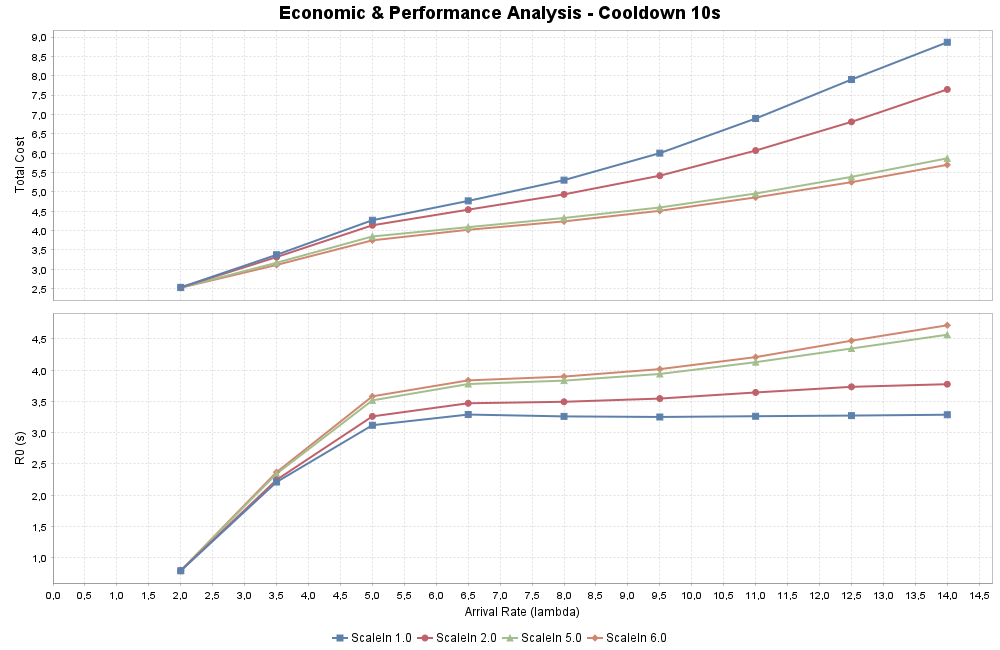
\includegraphics[width=\linewidth,height=.69\textheight,keepaspectratio]{../data/objective/cost/cost_analysis_cooldown_10s.png}
    \source{Costo aggregato e \(R_0\) per diverse soglie di Scale In, \(T_c=10\,s\).}
    \column{.35\textwidth}
    \textbf{Scelta equilibrata}
    \begin{itemize}
      \item \(R^{\min}=3.5\,s\);
      \item cooldown \(=10\,s\);
      \item costo medio \(=4.469\);
      \item SLA rispettato fino a \(\lambda=11\).
    \end{itemize}
    \vspace{0.3cm}
    {\small Soglie più basse riducono la latenza ma mantengono più server
      attivi. Un cooldown da \(100\,s\) reagisce troppo lentamente:
      nel caso peggiore \(R_0=6.3678\,s\).}
  \end{columns}
\end{frame}

% --------------------------------------------------------------------------
\begin{frame}{Costo: quando il controller diventa troppo lento}
  \begin{columns}[T,onlytextwidth]
    \column{.62\textwidth}
    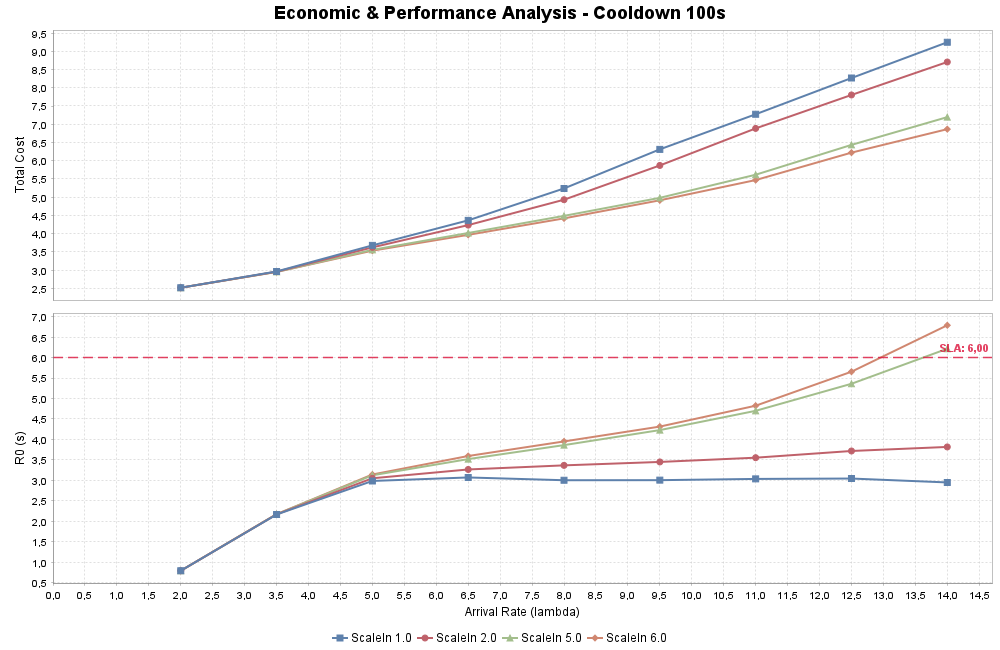
\includegraphics[width=\linewidth,height=.70\textheight,keepaspectratio]{../data/objective/cost/cost_analysis_cooldown_100s.png}
    \source{Costo e \(R_0\) con cooldown \(100\,s\).}
    \column{.35\textwidth}
    \tagbox{coral}{CASO CRITICO}\par\vspace{0.15cm}
    {\Large\bfseries \(R_0=6.3678\,s\)}
    \vspace{0.4cm}
    \begin{itemize}
      \item \(R^{\min}=5.0\,s\);
      \item carico massimo;
      \item reazione tardiva;
      \item SLA violato.
    \end{itemize}
    \vspace{0.35cm}
    \begin{block}{Conclusione}
      \(10\,s\) evita sia l'eccesso di riconfigurazioni del caso \(5\,s\),
      sia l'inerzia dei casi \(50\)--\(100\,s\).
    \end{block}
  \end{columns}
\end{frame}

% 10 -----------------------------------------------------------------------
\begin{frame}{Analisi del transitorio: il sistema si assesta}
  \begin{columns}[T,onlytextwidth]
    \column{.63\textwidth}
    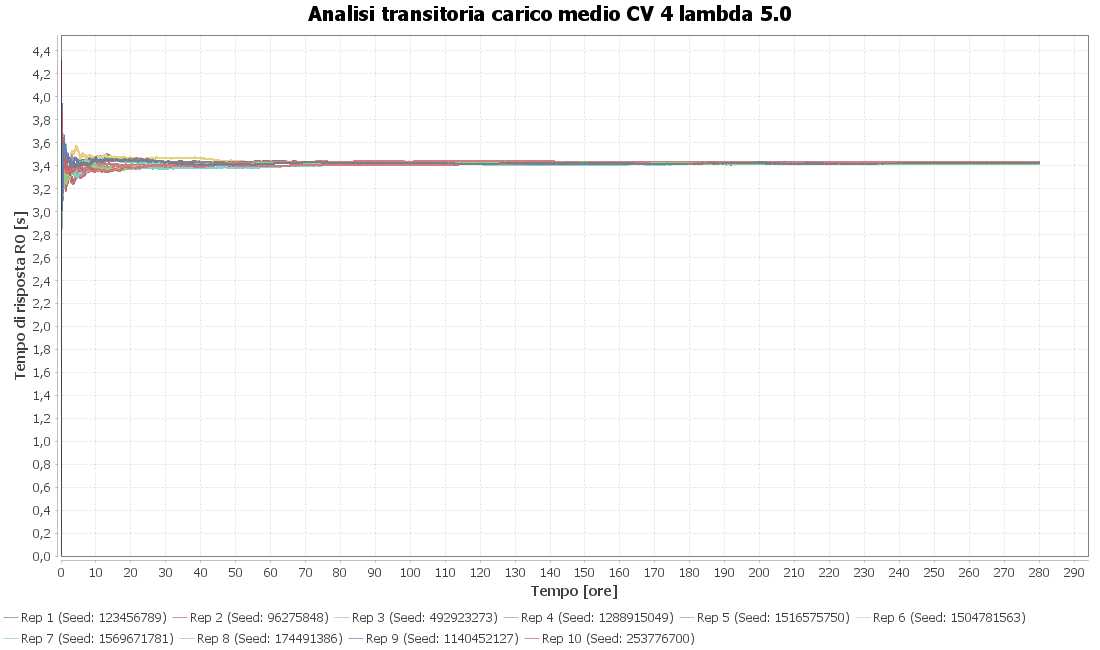
\includegraphics[width=\linewidth,height=.70\textheight,keepaspectratio]{../data/objective/finite/transient_medium_load_cv4.png}
    \source{Scenario medio: \(\lambda=5\) job/s, \(C_V=4\), sistema inizialmente vuoto.}
    \column{.34\textwidth}
    \textbf{Cosa osserviamo}
    \begin{itemize}
      \item nessuna deriva iniziale persistente;
      \item medie cumulative stabili;
      \item \(R_0\) sotto SLA in tutti i 6 scenari;
      \item ai carichi medio-alti cooperano entrambi i livelli.
    \end{itemize}
    \vspace{0.35cm}
    \begin{block}{Interpretazione}
      Il transitorio non invalida le conclusioni ottenute a regime.
    \end{block}
  \end{columns}
\end{frame}

% --------------------------------------------------------------------------
\begin{frame}{Transitorio: sei scenari, stesso esito}
  \begin{columns}[T,onlytextwidth]
    \column{.60\textwidth}
    \renewcommand{\arraystretch}{1.28}
    \begin{tabular}{@{}lrrrr@{}}
      \toprule
      \textbf{Scenario} & \(\lambda\) & \(C_V\) & \(R_0\,[s]\) & \textbf{Spike} \\
      \midrule
      Low CV2           & 2.5         & 2       & 0.8102       & 0.00\%         \\
      Low CV4           & 2.5         & 4       & 1.1721       & 0.00\%         \\
      Medium CV4        & 5.0         & 4       & 3.4112       & 9.97\%         \\
      Medium CV6        & 5.0         & 6       & 3.3106       & 14.72\%        \\
      High CV4          & 8.0         & 4       & 3.6842       & 40.28\%        \\
      High CV6          & 8.0         & 6       & 3.4626       & 43.07\%        \\
      \bottomrule
    \end{tabular}
    \column{.36\textwidth}
    \tagbox{green}{6 SU 6 SOTTO SLA}
    \vspace{0.45cm}
    \begin{itemize}
      \item a basso carico lo Spike resta spento;
      \item a carico medio assorbe i burst;
      \item ad alto carico supera il \(40\%\) di utilizzo;
      \item nessuna deriva tra le repliche.
    \end{itemize}
    \vspace{0.3cm}
    {\small Il sistema cambia \emph{come} usa le risorse, non perde
      stabilità.}
  \end{columns}
\end{frame}

% 12 -----------------------------------------------------------------------
\begin{frame}[shrink=3]{Burstiness: la gerarchia redistribuisce il carico}
  \begin{columns}[T,onlytextwidth]
    \column{.62\textwidth}
    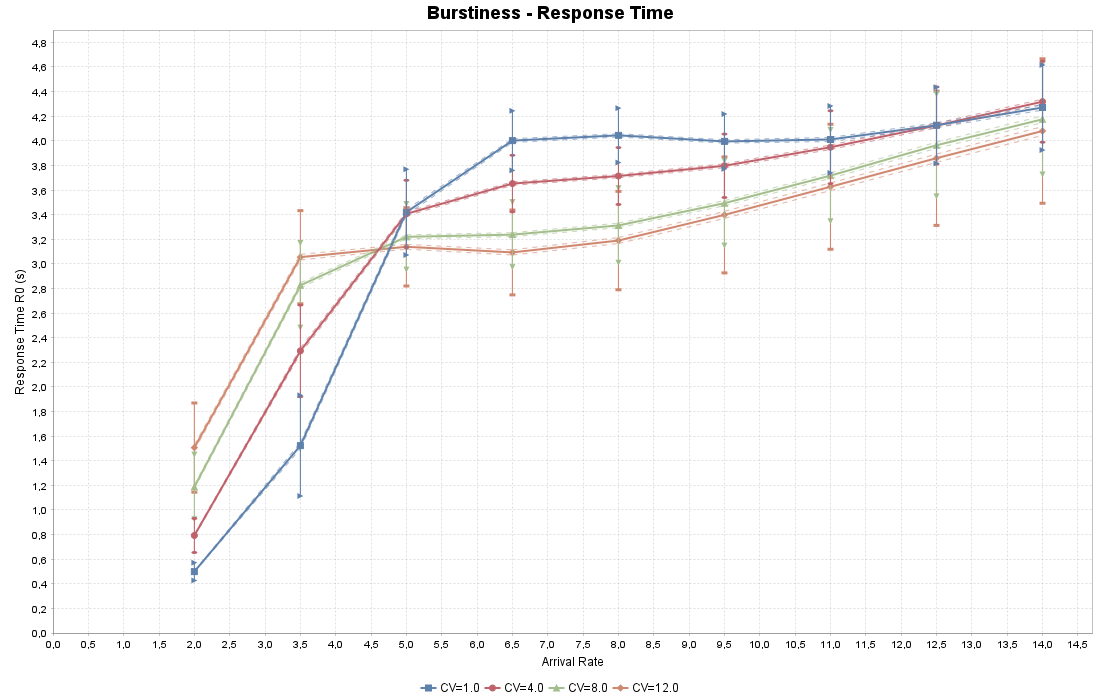
\includegraphics[width=\linewidth,height=.68\textheight,keepaspectratio]{../data/objective/burstiness/burstiness_robustness_response_time.png}
    \source{Tempo medio di risposta al variare di \(\lambda\) e \(C_V\).}
    \column{.35\textwidth}
    \begin{center}
      {\color{coral}\bfseries\large \(4.2853\,s\)}\par
      {\scriptsize\color{muted}massimo \(R_0\) osservato}
    \end{center}
    \vspace{0.5cm}

    \begin{itemize}
      \item tutta la griglia resta sotto SLA;
      \item a \(\lambda=5\), i burst attivano entrambi gli scaler;
      \item a \(\lambda=11\), il pool ordinario cresce e alleggerisce lo Spike Server.
    \end{itemize}
    \vspace{0.25cm}
    {\small Per \(\lambda=11\), passando da \(C_V=1\) a \(12\),
      l'utilizzazione Spike scende dal \(68.18\%\) al \(59.19\%\).}
  \end{columns}
\end{frame}

% --------------------------------------------------------------------------
\begin{frame}{Burstiness: chi assorbe davvero il carico?}
  \begin{columns}[T,onlytextwidth]
    \column{.49\textwidth}
    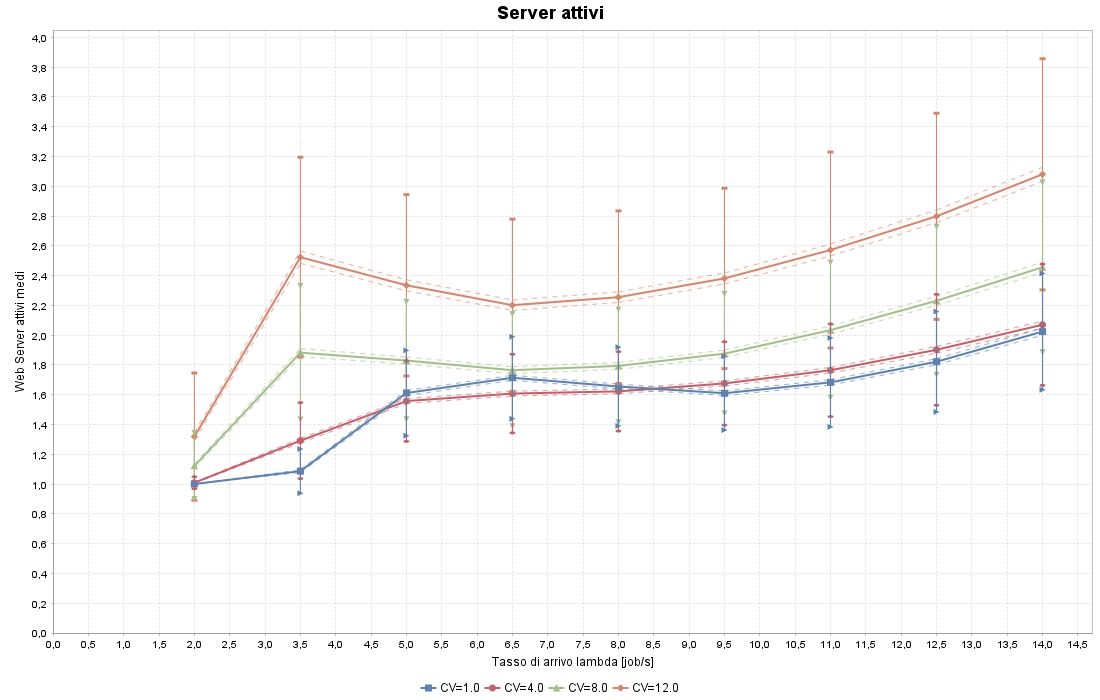
\includegraphics[width=\linewidth,height=.58\textheight,keepaspectratio]{../data/objective/burstiness/burstiness_robustness_avg_servers.png}
    \begin{center}\tagbox{teal}{WEB SERVER ATTIVI}\end{center}
    \column{.49\textwidth}
    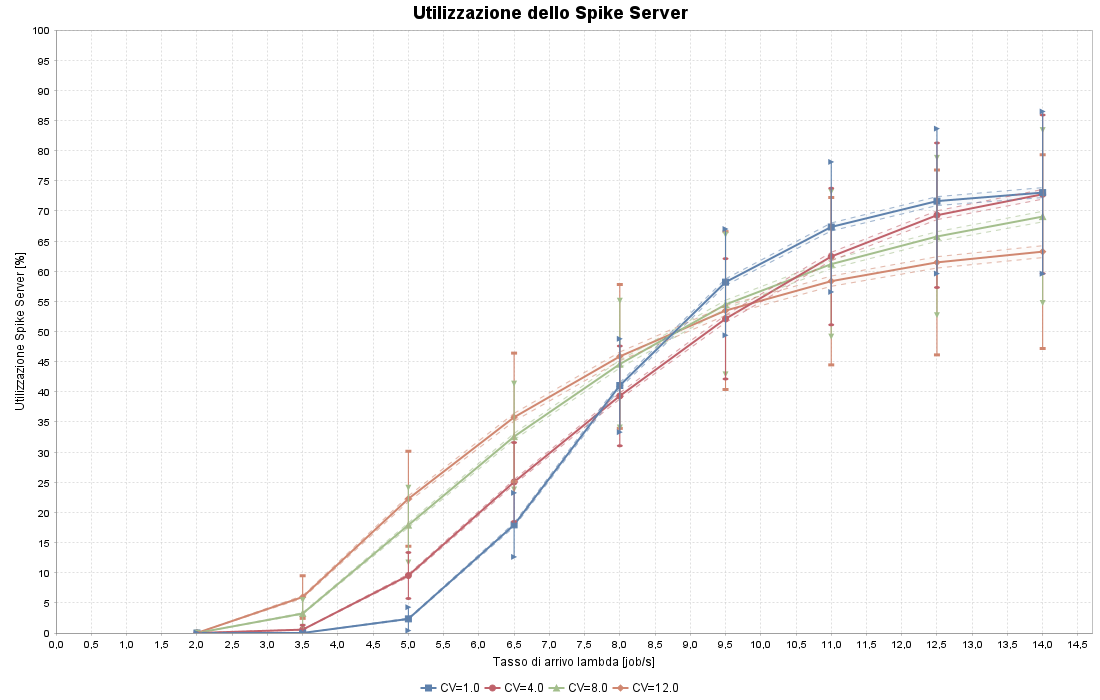
\includegraphics[width=\linewidth,height=.58\textheight,keepaspectratio]{../data/objective/burstiness/burstiness_robustness_spike_utilization.png}
    \begin{center}\tagbox{coral}{UTILIZZO SPIKE}\end{center}
  \end{columns}
  \vspace{0.15cm}
  \begin{center}
    {\small A \(\lambda=5\) crescono entrambi. A \(\lambda=11\), il pool
      ordinario più ampio riduce il ricorso proporzionale allo Spike Server.}
  \end{center}
\end{frame}

% --------------------------------------------------------------------------
\begin{frame}{Burstiness: il controllo reagisce, il flusso resta stabile}
  \begin{columns}[T,onlytextwidth]
    \column{.49\textwidth}
    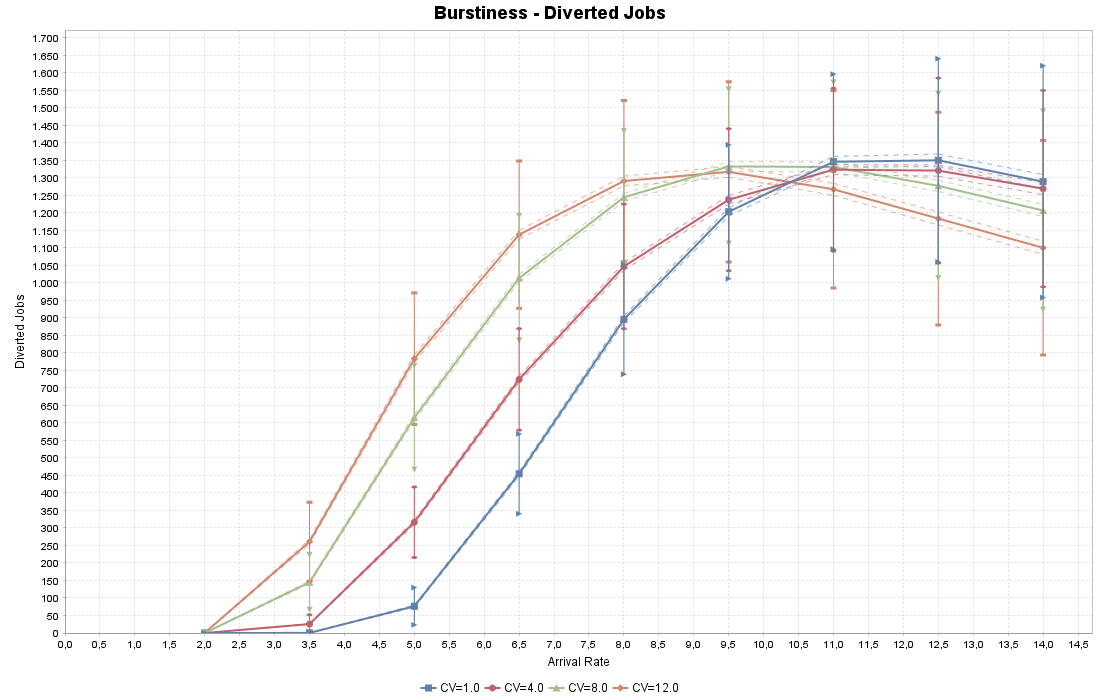
\includegraphics[width=\linewidth,height=.58\textheight,keepaspectratio]{../data/objective/burstiness/burstiness_robustness_diverted_jobs.png}
    \begin{center}\tagbox{coral}{JOB DEVIATI}\end{center}
    \column{.49\textwidth}
    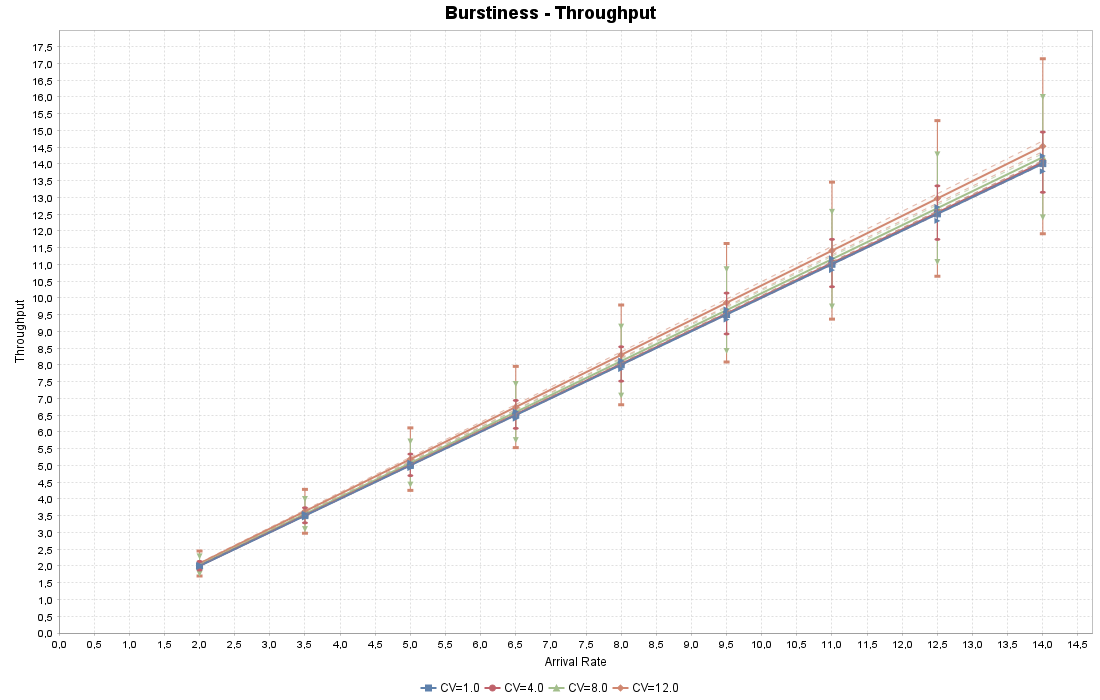
\includegraphics[width=\linewidth,height=.58\textheight,keepaspectratio]{../data/objective/burstiness/burstiness_robustness_throughput.png}
    \begin{center}\tagbox{teal}{THROUGHPUT}\end{center}
  \end{columns}
  \vspace{0.15cm}
  \begin{center}
    {\small Più variabilità produce più interventi e più deviazioni,
      ma non perdita di throughput né instabilità delle metriche.}
  \end{center}
\end{frame}

% 13 -----------------------------------------------------------------------
\begin{frame}{Limite del modello base: chattering vicino alla soglia}
  \begin{columns}[T,onlytextwidth]
    \column{.51\textwidth}
    \begin{tikzpicture}[x=.095cm,y=.105cm]
      \draw[->,muted,thick] (0,0)--(61,0) node[right,font=\scriptsize]{tempo};
      \draw[->,muted,thick] (0,0)--(0,47) node[above,font=\scriptsize]{\(SI_i\)};
      \draw[coral,dashed,thick] (0,40)--(59,40);
      \node[coral,font=\scriptsize\bfseries,anchor=south east] at (59,40) {\(SI_{\max}\)};
      \draw[ink,very thick] plot coordinates {
          (0,34)(8,38)(14,41)(20,39)(27,42)(34,38)(41,41)(48,39)(56,43)};
      \foreach \x/\c in {14/coral,20/teal,27/coral,34/teal,41/coral,48/teal,56/coral}
      \fill[\c] (\x,{ifthenelse(\x==20 || \x==34 || \x==48,39,41)}) circle (1.2);
    \end{tikzpicture}
    \column{.45\textwidth}
    Con una soglia rigida, piccole oscillazioni producono continui
    cambi di destinazione.
    \vspace{0.4cm}

    \begin{block}{Miglioramento: banda}
      Ogni Web Server mantiene uno stato:
      \[
        B=SI_{\max}-SI_{\text{low}}.
      \]
      Si entra in modalità spike a \(SI_{\max}\), ma si rientra nel percorso
      ordinario solo a \(SI_{\text{low}}\).
    \end{block}
    \vspace{0.2cm}
    {\small La memoria stabilizza il controllo, al prezzo di una maggiore
      permanenza sullo Spike Server.}
  \end{columns}
\end{frame}

% --------------------------------------------------------------------------
\begin{frame}{Meccanismo a bande: verifica trace-driven}
  \begin{columns}[T,onlytextwidth]
    \column{.68\textwidth}
    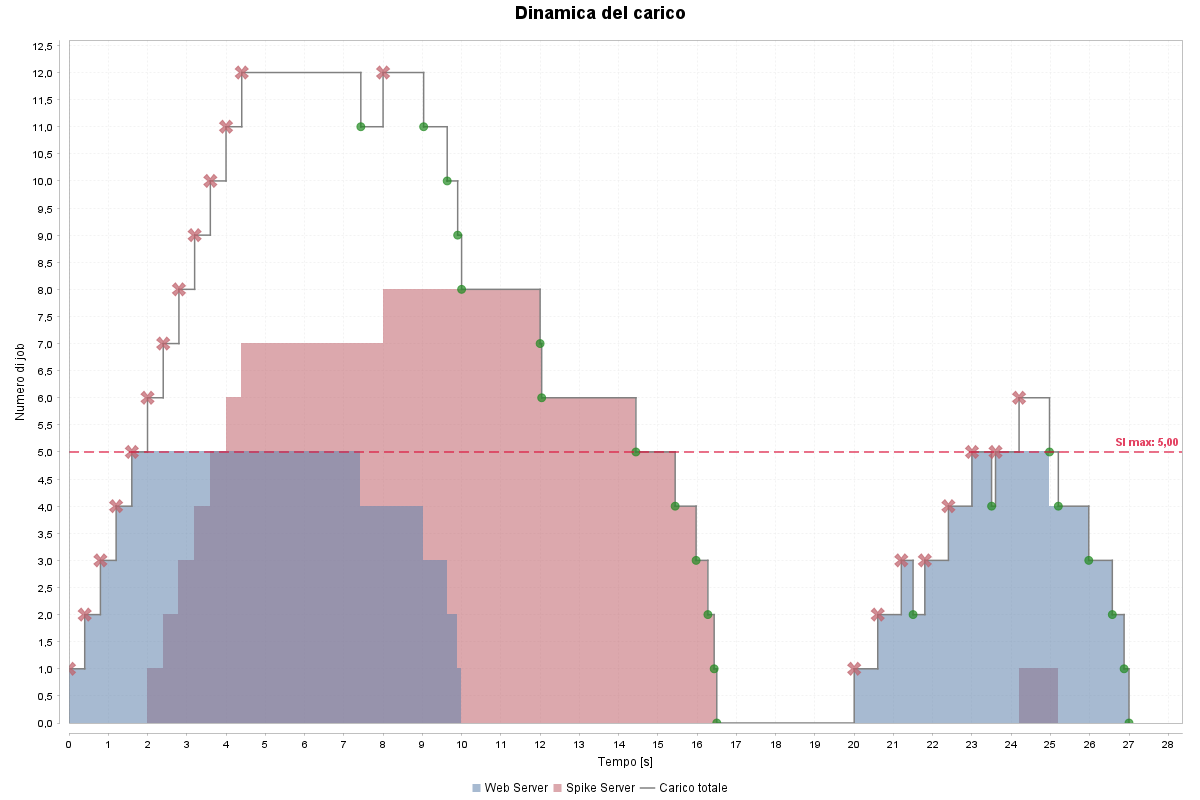
\includegraphics[width=\linewidth,height=.70\textheight,keepaspectratio]{../data/vv/chart/band_diversion_chart.png}
    \source{\(SI_{\max}=5\), \(SI_{\mathrm{low}}=2\), 21 arrivi deterministici.}
    \column{.29\textwidth}
    \tagbox{teal}{COMPORTAMENTO ATTESO}
    \vspace{0.35cm}
    \begin{itemize}
      \item attivazione a \(SI_{\max}\);
      \item persistenza nella banda;
      \item rilascio solo a \(SI_{\mathrm{low}}\);
      \item nuova attivazione corretta.
    \end{itemize}
    \vspace{0.3cm}
    {\small Nessun rientro prematuro, nessun job perso.}
  \end{columns}
\end{frame}

% 14 -----------------------------------------------------------------------
\begin{frame}{Sistema modificato: meno latenza, più uso dello spike}
  \begin{columns}[T,onlytextwidth]
    \column{.58\textwidth}
    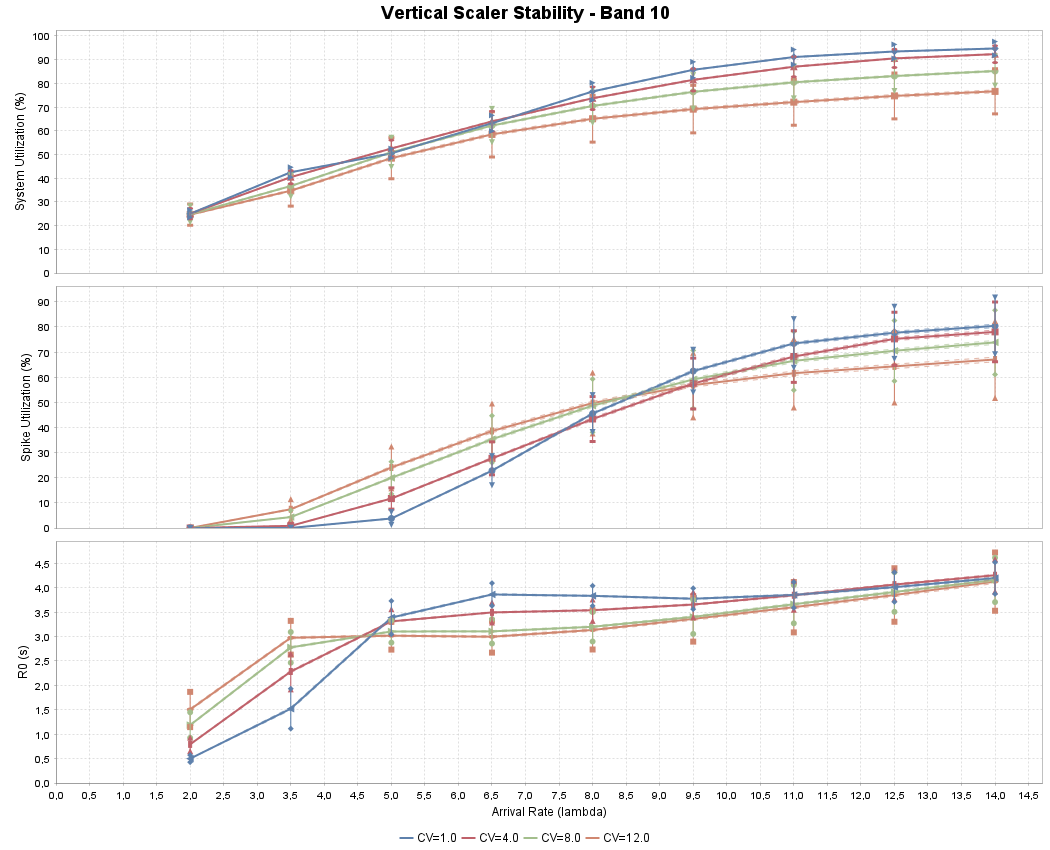
\includegraphics[width=\linewidth,height=.68\textheight,keepaspectratio]{../data/objective/band/vertical_scaler_stability_band_10.png}
    \source{Banda \(B=10\): utilizzazioni e tempo di risposta al variare del carico.}
    \column{.39\textwidth}
    \begin{center}
    \renewcommand{\arraystretch}{1.25}
    \begin{tabular}{@{}lrr@{}}
      \toprule
                         & \(B=0\) & \(B=10\) \\
      \midrule
      \(R_0,\lambda=5\)  & 3.3939  & 3.3116   \\
      Spike util.        & 9.91\%  & 11.73\%  \\
      \(R_0,\lambda=11\) & 3.9401  & 3.8465   \\
      Spike util.        & 63.47\% & 68.21\%  \\
      \bottomrule
    \end{tabular}
    \vspace{0.4cm}

    \begin{block}{Scelta finale}
      \(B=10\) è il compromesso: a \(\lambda=11\) riduce la latenza del
      \(2.4\%\) con \(+4.7\) punti di utilizzazione Spike.
    \end{block}
    \end{center}
  \end{columns}
\end{frame}

% --------------------------------------------------------------------------
\begin{frame}{Ampiezza della banda: quattro punti sul trade-off}
  \begin{columns}[T,onlytextwidth]
    \column{.57\textwidth}
    \begin{center}
    \renewcommand{\arraystretch}{1.32}
    \begin{tabular}{@{}rrrrr@{}}
      \toprule
      \(B\) & \(R_0\) \(\lambda=5\) & Spike   & \(R_0\) \(\lambda=11\) & Spike   \\
      \midrule
      0     & 3.3939                & 9.91\%  & 3.9401                 & 63.47\% \\
      5     & 3.3599                & 10.65\% & 3.8993                 & 65.46\% \\
      10    & 3.3116                & 11.73\% & 3.8465                 & 68.21\% \\
      20    & 3.1766                & 13.54\% & 3.7576                 & 74.46\% \\
      \bottomrule
    \end{tabular}
    \par\vspace{0.55cm}
      \begin{minipage}{.86\linewidth}
        \centering
        {\small Gli intervalli delle configurazioni estreme non si
        sovrappongono: il beneficio non è rumore statistico.}
      \end{minipage}
    \end{center}
    \column{.39\textwidth}
    \tagbox{gold}{B=20}\par
    Latenza minima, ma \(+11\) punti di utilizzo Spike a \(\lambda=11\).
    \vspace{0.5cm}

    \tagbox{teal}{B=10}\par
    Riduzione del \(2.4\%\) di \(R_0\), con \(+4.7\) punti di utilizzo.
    \vspace{0.5cm}

    \begin{block}{Scelta}
      \(B=10\): miglior compromesso prestazioni--costo.
    \end{block}
  \end{columns}
\end{frame}

% 15 -----------------------------------------------------------------------
\begin{frame}{Conclusioni}
  \begin{columns}[T,onlytextwidth]
    \column{.63\textwidth}
    \begin{enumerate}
      \item \textbf{Due scale temporali richiedono due forme di elasticità.}
            Lo scaling orizzontale segue il trend; lo Spike Server assorbe i burst.
            \vspace{0.28cm}
      \item \textbf{La simulazione rende esplicito il trade-off.}
            \(SI_{\max}=40\), \(R^{\min}=3.5\,s\) e cooldown \(10\,s\) rispettano
            lo SLA senza sovradimensionare il sistema.
            \vspace{0.28cm}
      \item \textbf{La memoria migliora la stabilità.}
            Una banda \(B=10\) riduce il chattering e la latenza con un costo
            operativo controllato.
    \end{enumerate}
    \column{.33\textwidth}
    \vspace{0.2cm}
    \begin{tikzpicture}
      \node[circle,fill=teal,text=white,minimum size=2.2cm,
        align=center,font=\bfseries] (a) {SLA\\rispettato};
      \node[circle,fill=coral,text=white,minimum size=1.7cm,
        align=center,font=\small\bfseries,below right=-.25cm and -.05cm of a] {costo\\controllato};
      \node[circle,fill=gold,text=ink,minimum size=1.55cm,
        align=center,font=\small\bfseries,below left=-.15cm and -.12cm of a] {routing\\stabile};
    \end{tikzpicture}
  \end{columns}
  \vfill
  \begin{center}
    {\Large\bfseries\color{ink}Grazie per l'attenzione}
  \end{center}
\end{frame}

\end{document}
